\documentclass[10pt]{beamer}

\usepackage[utf8]{inputenc}
\usepackage[T1]{fontenc}
\usepackage[frenchb]{babel}
\usepackage{amssymb}
\usepackage{amsmath}
\usepackage{bm}
\usepackage{tikz}
\usepackage{mathrsfs}
\usepackage{graphicx}
\usepackage{verbatim}
\usepackage{multimedia}

\title[Correction défauts robots humanoïdes]{
Apprentissage et correction des imperfections 
des robots humanoïdes de petite taille :\\
application à l'odométrie et à la synthèse de mouvements
}
\author[Quentin Rouxel]{
Quentin Rouxel\\
\vspace{0.1cm}
\small
Directeurs : Olivier Ly et Hugo Gimbert
}
\institute[Rhoban]{Équipe Rhoban - LaBRI - Université de Bordeaux}
\date[4 décembre 2017 (Thèse)]{Soutenance de thèse -- 4 décembre 2017}

%Beamer theme
\usetheme{Madrid}
%\usetheme{AnnArbor}
\usecolortheme{beaver}
\useinnertheme{circles}
\setbeamertemplate{blocks}[default]
\setbeamertemplate{blocks}[rounded][shadow=false]
%\setbeamertemplate{caption}[numbered]
%\setbeameroption{show notes}
%\setbeamercovered{transparent}

%Custom colors
\definecolor{UBXBleu}{RGB}{0,157,224}
\definecolor{UBXBleuLight}{RGB}{222,237,252}
\definecolor{UBXMarron}{RGB}{68,58,49}
\definecolor{UBXGris}{RGB}{232,232,232}
\setbeamercolor*{structure}{bg=white,fg=UBXBleu}
\setbeamercolor*{palette primary}{use=structure,fg=UBXMarron,bg=UBXGris}
\setbeamercolor*{palette secondary}{use=structure,fg=UBXMarron,bg=UBXBleuLight}
\setbeamercolor*{palette tertiary}{use=structure,fg=white,bg=UBXBleu}
\setbeamercolor{titlelike}{fg=white,bg=UBXBleu}
\setbeamercolor{frametitle}{bg=UBXGris,fg=UBXMarron}
\setbeamercolor{block title}{bg=UBXBleu,fg=white}
\setbeamercolor{block body}{bg=UBXBleuLight,fg=black}

%\setbeamercolor{frametitle}{bg=UBXBleu,fg=white}
%\setbeamercolor{block title}{bg=UBXGris,fg=UBXMarron}

%Disable presentation navigation buttons
\beamertemplatenavigationsymbolsempty

%Commande custom pour l'affochage des références
\newcommand{\customtextcolor}[1]{\usebeamercolor[fg]{structure}{#1}\usebeamercolor[fg]{normal text}}

% Macro pour la transposée
\newcommand\T{\mathsf{T}}

\begin{document}

\begin{frame}{}
    \begin{columns}
        \begin{column}{0.22\textwidth}
            
\includegraphics[width=0.7\linewidth]{../media/rhoban_logo.png}
        \end{column}
        \begin{column}{0.22\textwidth}
            
\includegraphics[width=\linewidth]{../media/logo_labri.jpg}
        \end{column}
        \begin{column}{0.22\textwidth}
            
\includegraphics[width=\linewidth]{../template/logo_ubx.jpg}
        \end{column}
        \begin{column}{0.22\textwidth}
            
\includegraphics[width=\linewidth]{../media/logo_inp.jpg}
        \end{column}
    \end{columns}
    \titlepage
\end{frame}

\section{Introduction}

\begin{frame}{Plan}
    \tableofcontents[ 
        sectionstyle=show, 
        subsectionstyle=show, 
        currentsubsection, 
        hideothersubsections, 
    ] 
\end{frame}


\subsection{RoboCup}

\begin{frame}{La compétition RoboCup (1/2) -- Origine et ambition}
    \begin{columns}
        \begin{column}{0.45\linewidth}
            \begin{block}{RoboCup}
                Compétition internationale
            \end{block}
            \begin{block}{Ambition -- 2050}
                Battre la meilleure équipe humaine de football
            \end{block}
            \vspace{1.0em}
            \begin{itemize}
                \setlength\itemsep{1.0em}
                \item Origine (1997) : victoire
                    aux échecs contre Garry Kasparov
                \item $\Rightarrow$ Grand défi pour l'IA
            \end{itemize}
        \end{column}
        \begin{column}{0.55\linewidth}
            \centering
            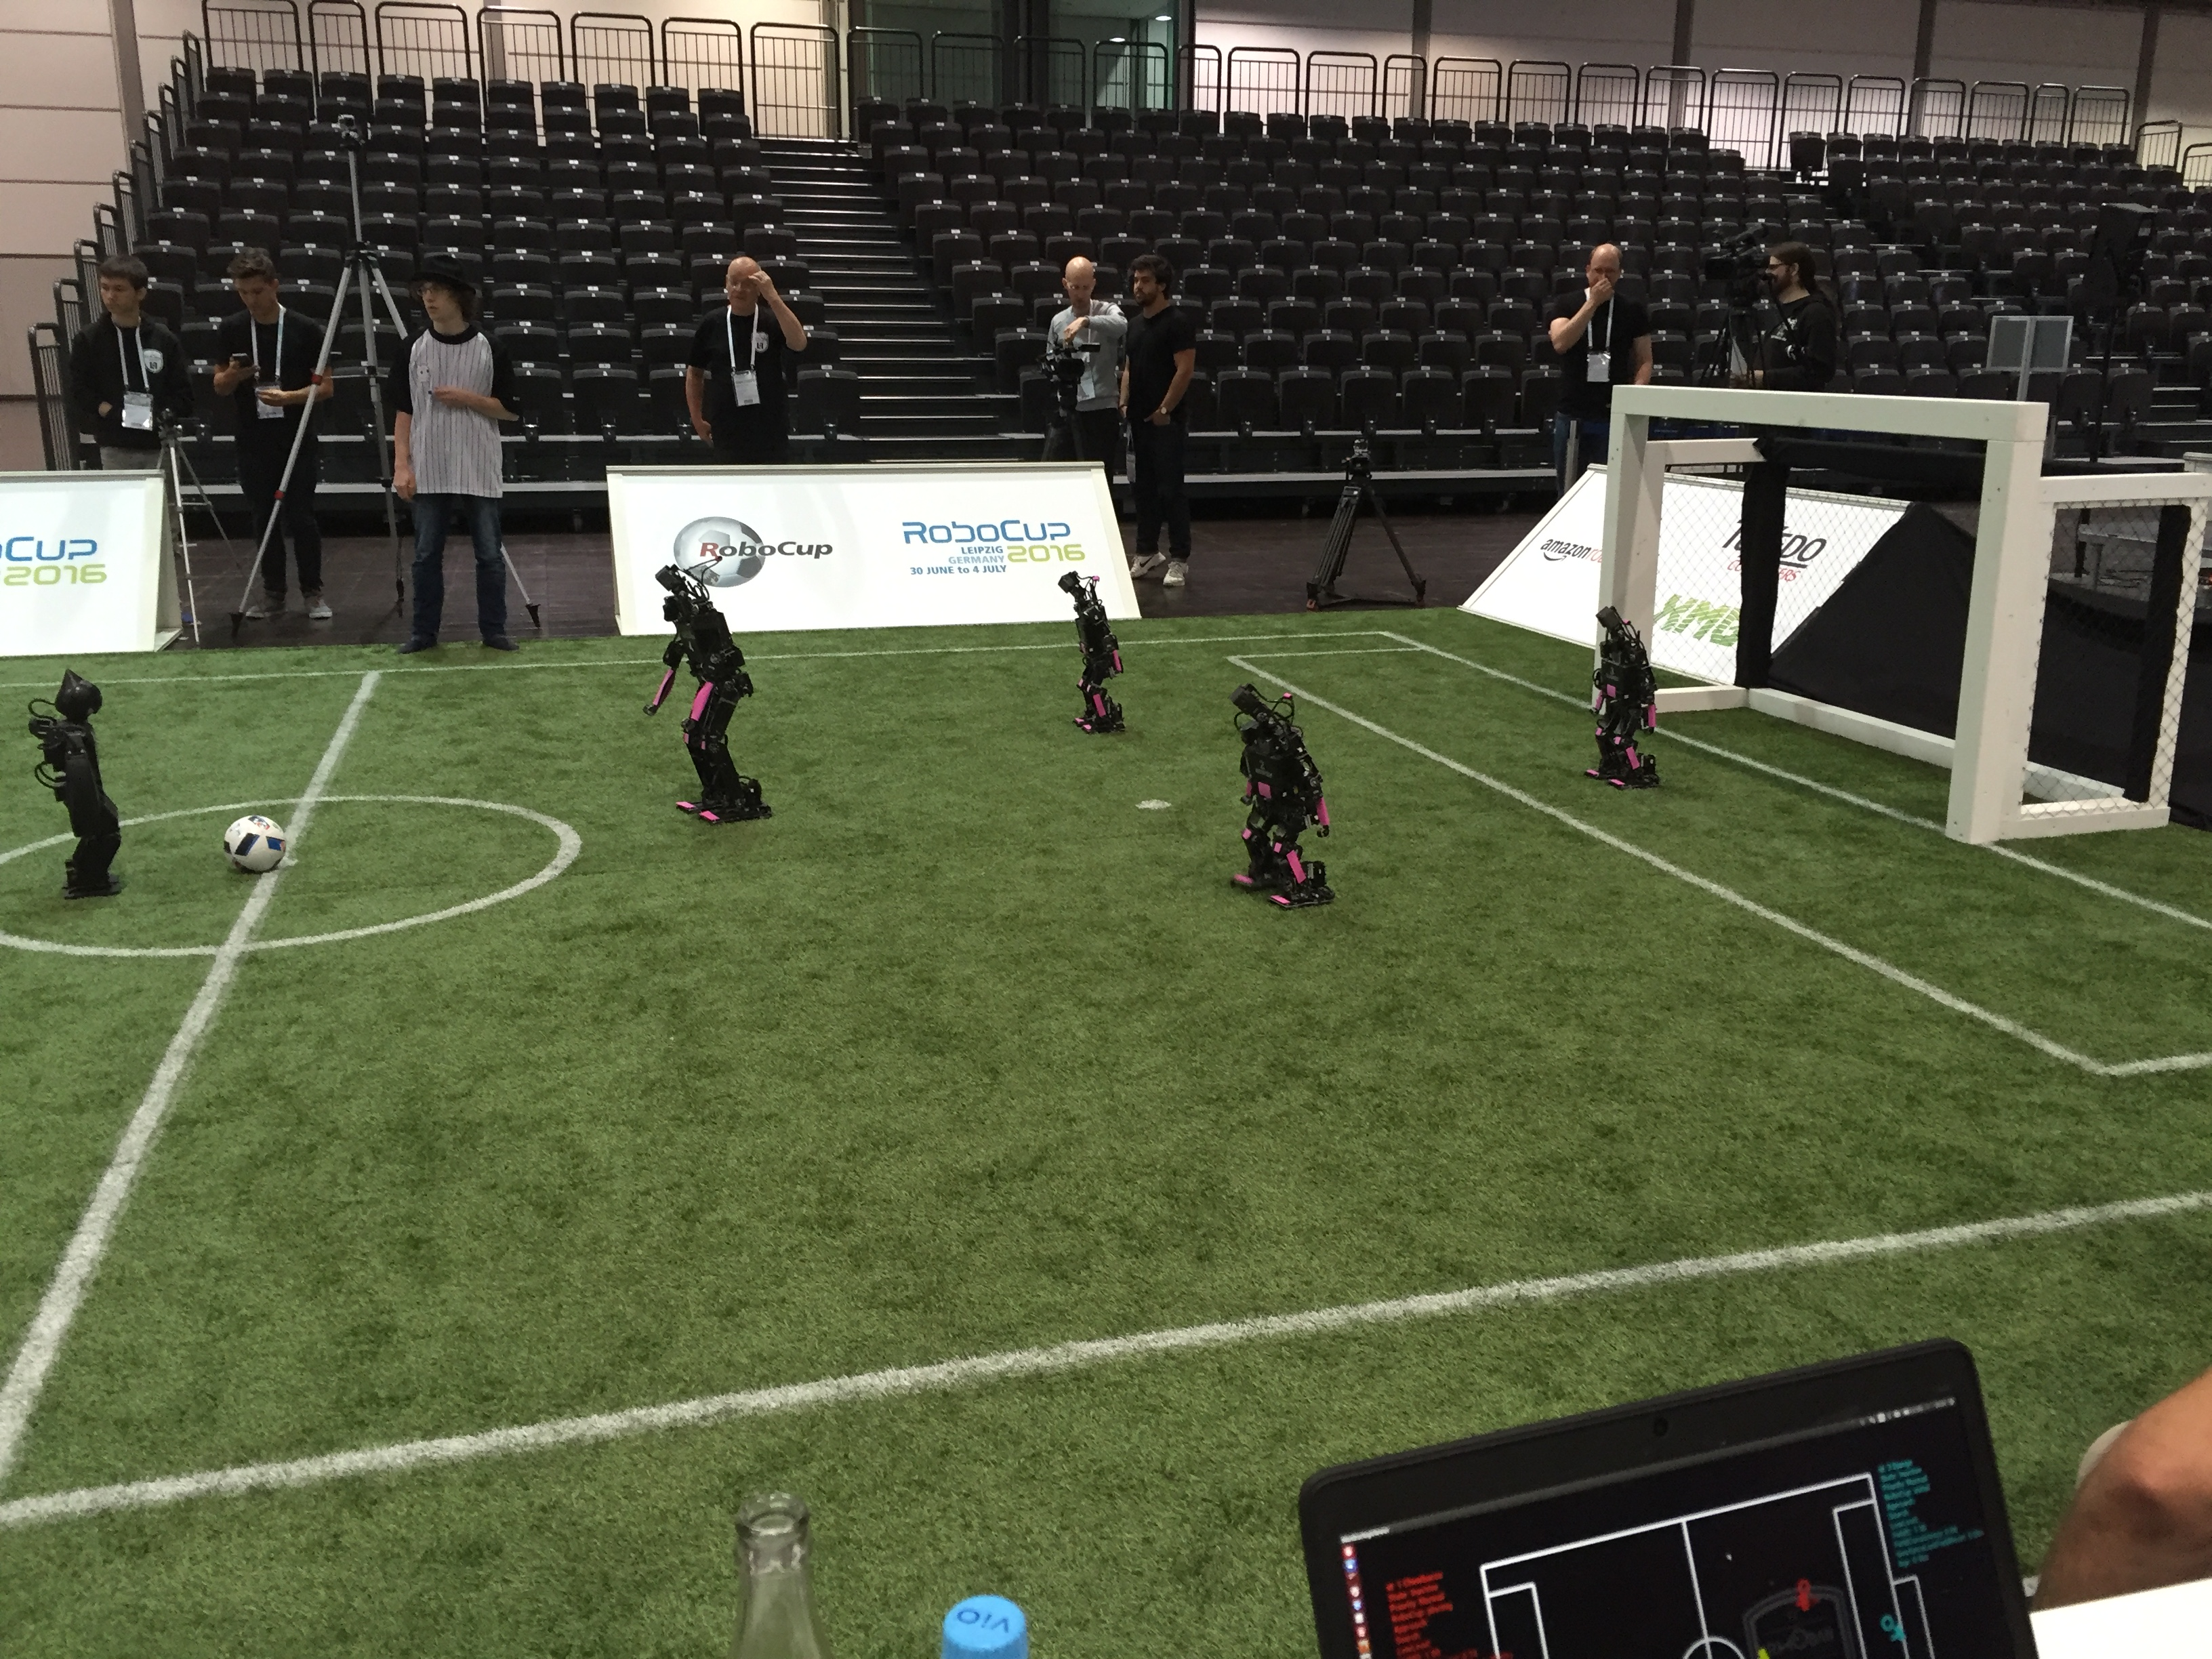
\includegraphics[width=1.0\linewidth]{../media/robocup_field.jpg}
        \end{column}
    \end{columns}
\end{frame}

\begin{frame}{La compétition RoboCup (2/2) -- Ligue \textit{Humanoid}}
    \begin{columns}
        \begin{column}{0.45\linewidth}
            3 tailles : 
            \textit{Kid-Size}, \textit{Teen-Size}, \textit{Adult-Size}\\
            \vspace{1.0em}
            \begin{block}{Ligue \textit{Humanoid Kid-Size}}
                Robots autonomes, anthropomorphe et non standards
            \end{block}
            \begin{itemize}
                \item Recherche : 
                    mécatronique, mouvements, perception
                \item Contraintes opérationnelles
            \end{itemize}
            \vspace{1.0em}
            \textit{Rhoban Football Club} : 
            1ère place \textit{Humanoid Kid-Size} en 2016 et 2017\\
        \end{column}
        \begin{column}{0.55\linewidth}
            \centering
            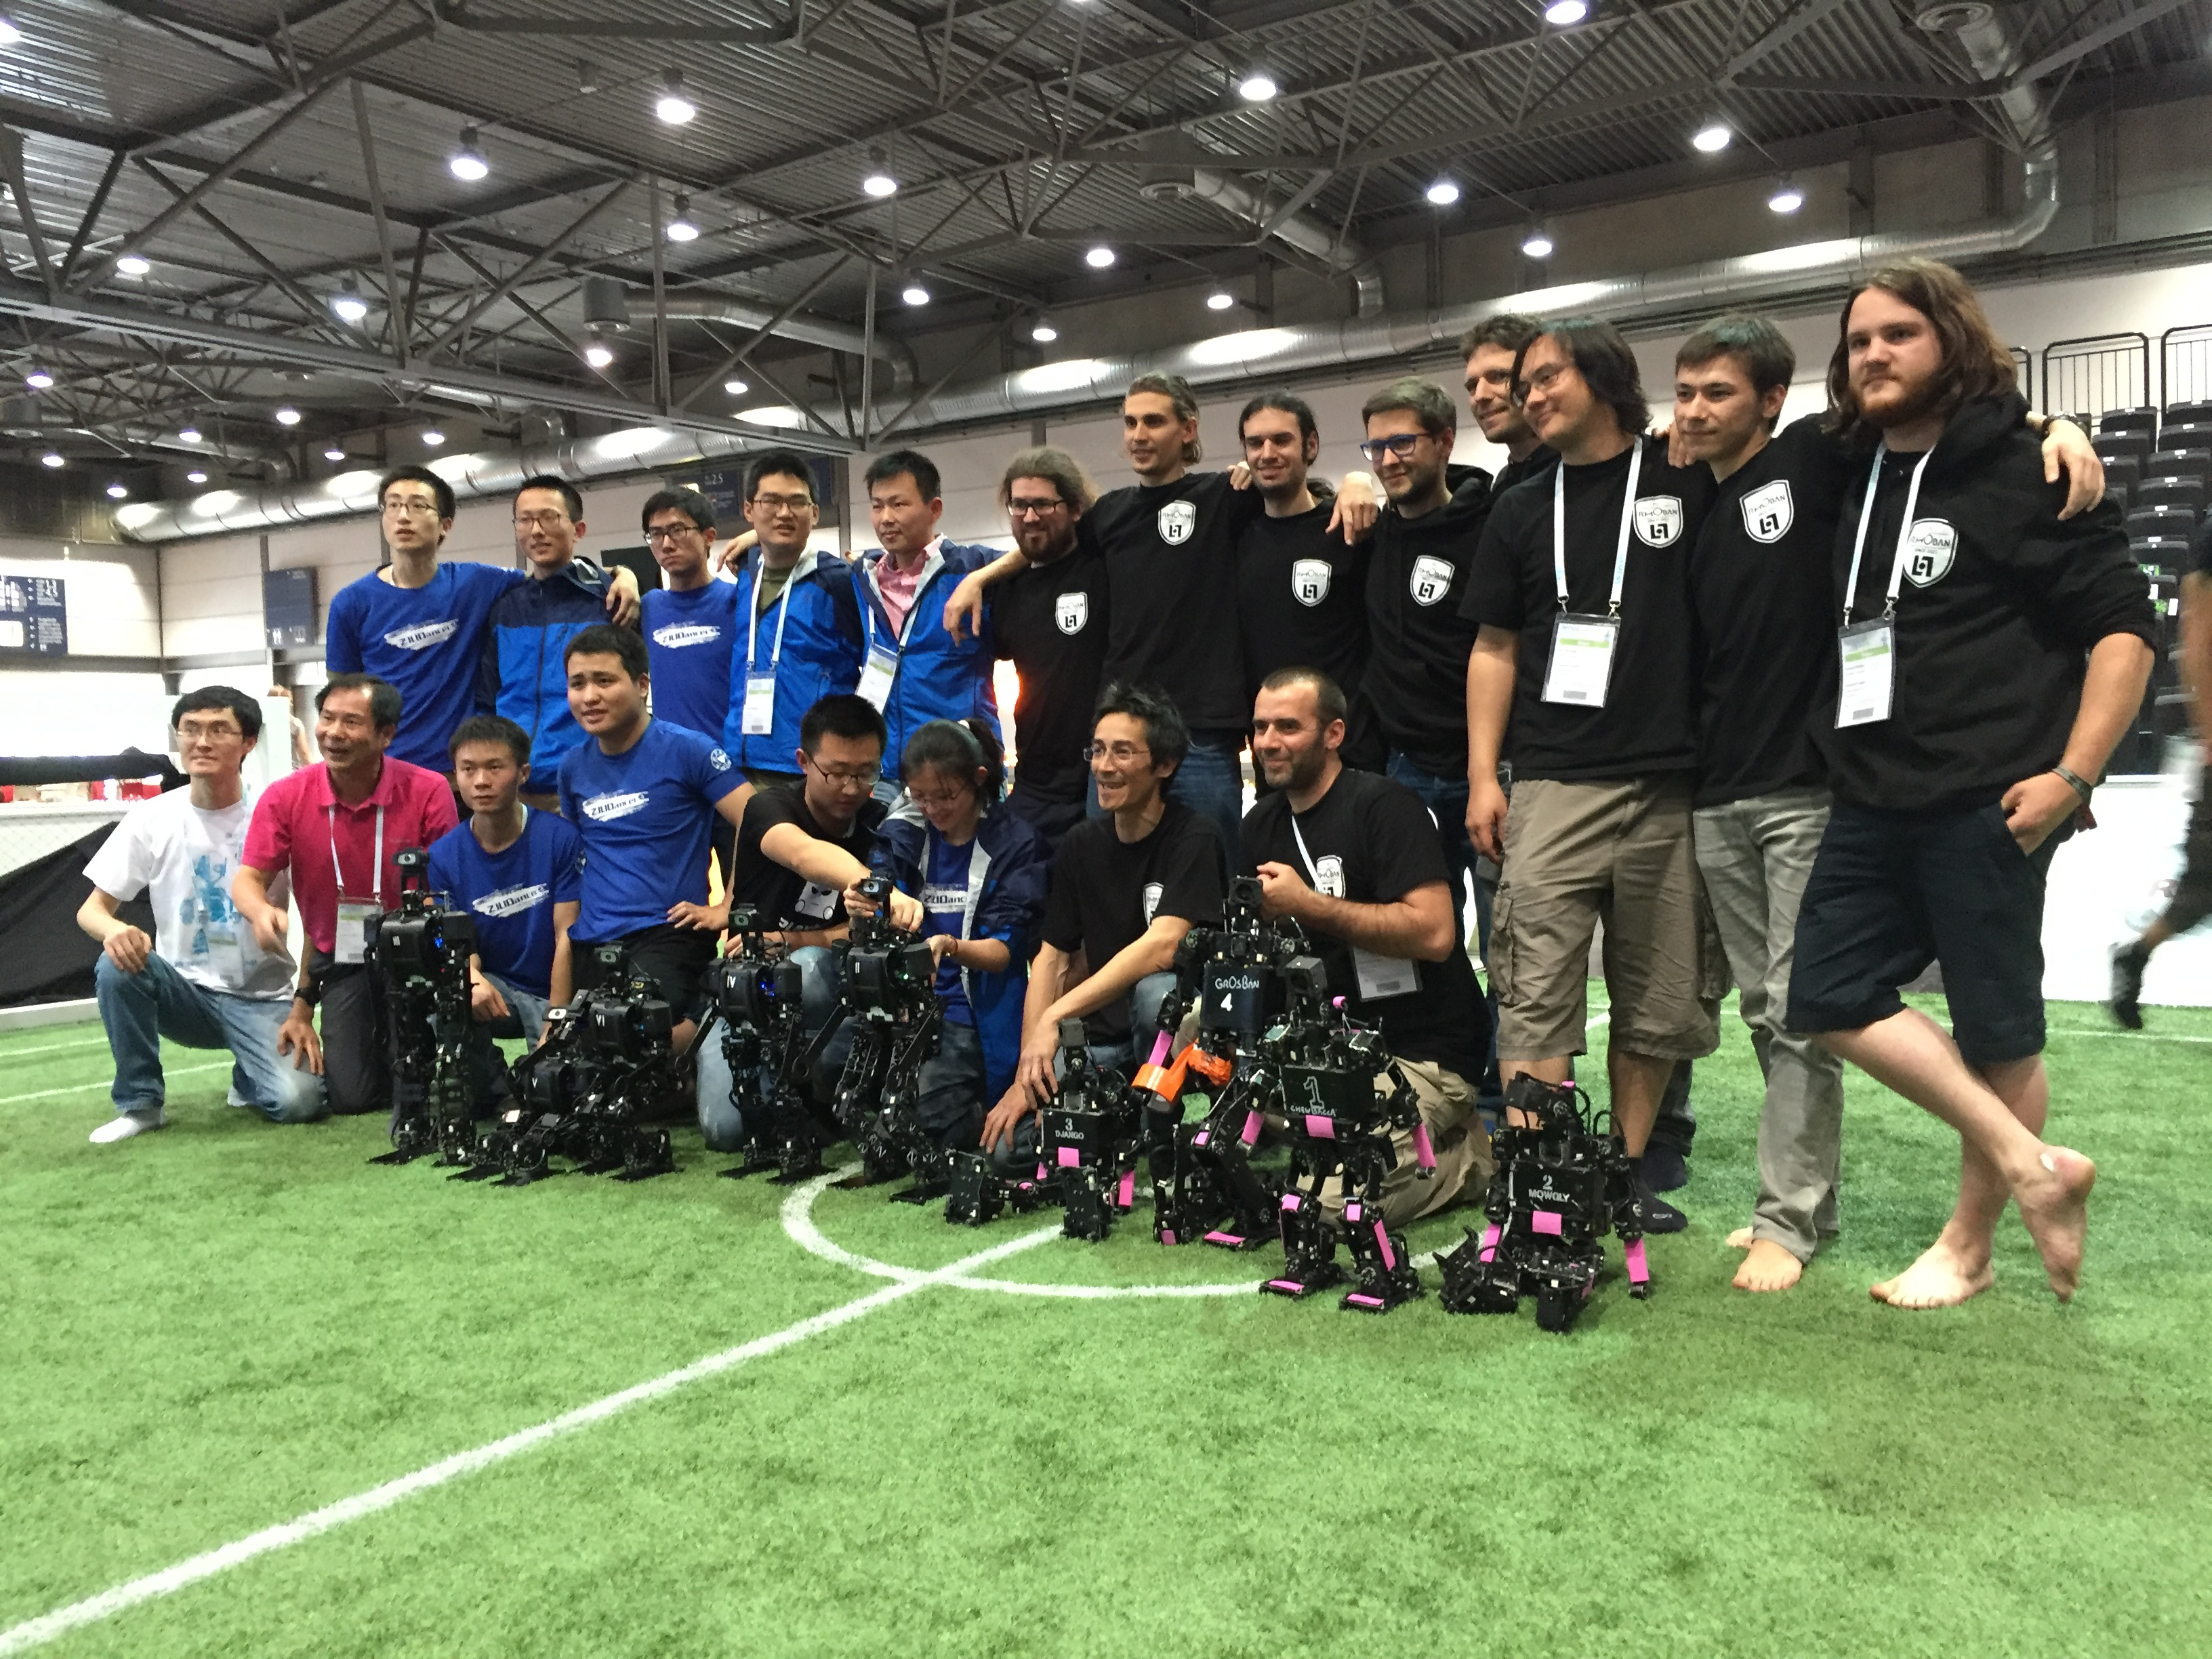
\includegraphics[width=1.0\linewidth]{../media/robocup_team.jpg}
        \end{column}
    \end{columns}
    \begin{block}{}
        \customtextcolor{
            \small
            \textit{Rhoban football club: Robocup humanoid kid-size 2016 champion team paper}}\\
        \scriptsize
        Julien Allali, Louis Deguillaume, Rémi Fabre, Loic Gondry, Ludovic Hofer, Olivier Ly, 
        Steve N'Guyen, Grégoire Passault, Antoine Pirrone, Quentin Rouxel\\
        RoboCup 2016\\
    \end{block}
\end{frame}


\subsection{Plateforme robotique}

\begin{frame}{Le robot Sigmaban (1/2) -- Caractéristiques matérielles}
    \begin{columns}
        \begin{column}{0.32\linewidth}
            Robot humanoïde Sigmaban :
            \begin{itemize}
                \item Taille : $57$~cm
                \item Poids : $4.2$~Kg
                \item Articulations : $20$
                \vspace{1.0em}
                \item Caméra industrielle
                \item Processeur x86
                \item IMU (accéléromètres, gyromètres)
                \item Capteurs de pression
                \item Servomoteurs Dynamixel
            \end{itemize}
        \end{column}
        \begin{column}{0.6\linewidth}
            \begin{columns}
                \begin{column}{0.4\linewidth}
                    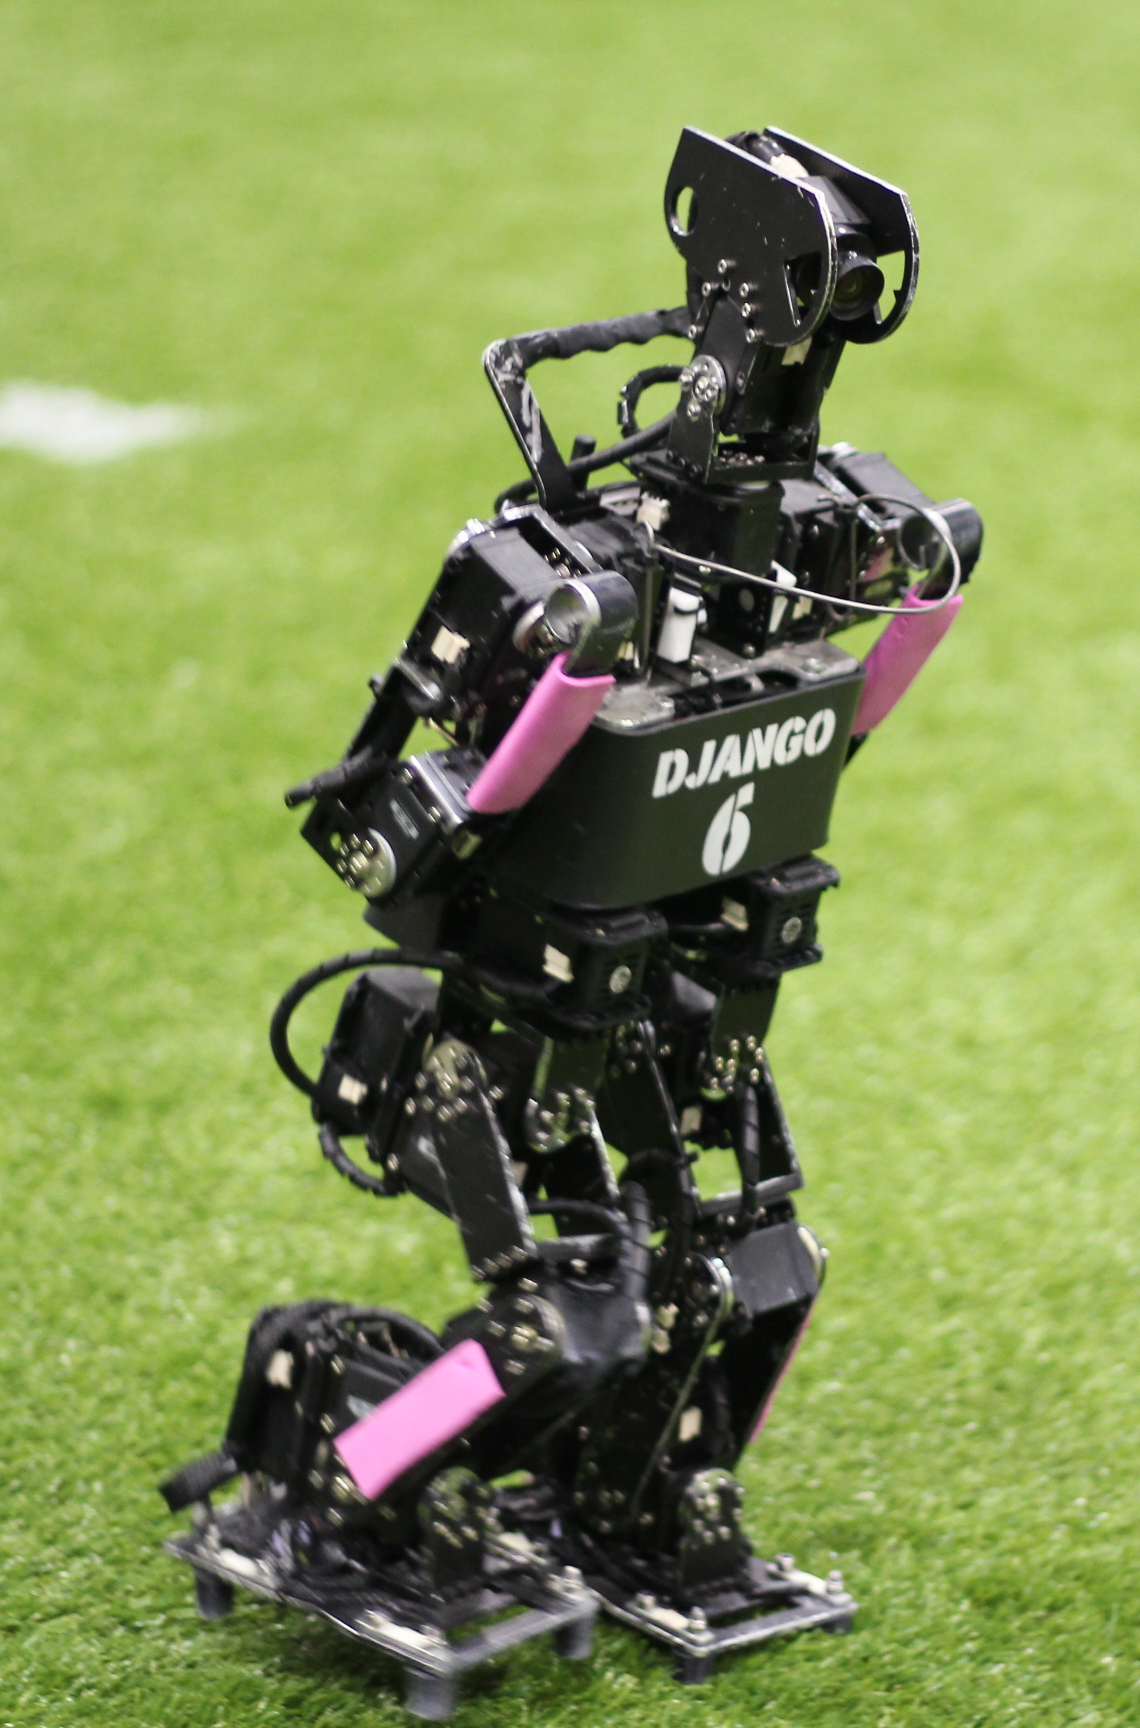
\includegraphics[width=1.0\linewidth]{../media/sigmaban_1_6.png}
                \end{column}
                \begin{column}{0.6\linewidth}
                    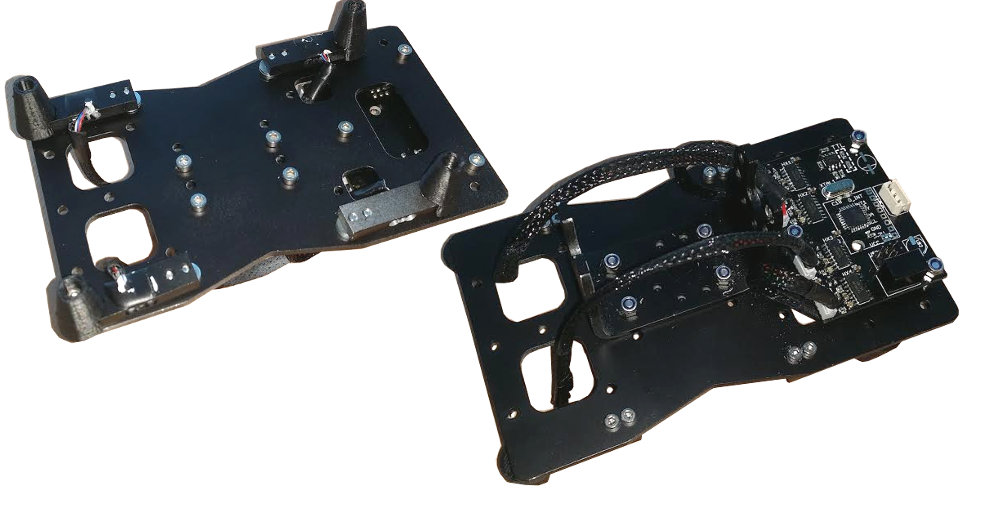
\includegraphics[width=1.1\linewidth]{../media/pressures2.png}
                    \newline
                    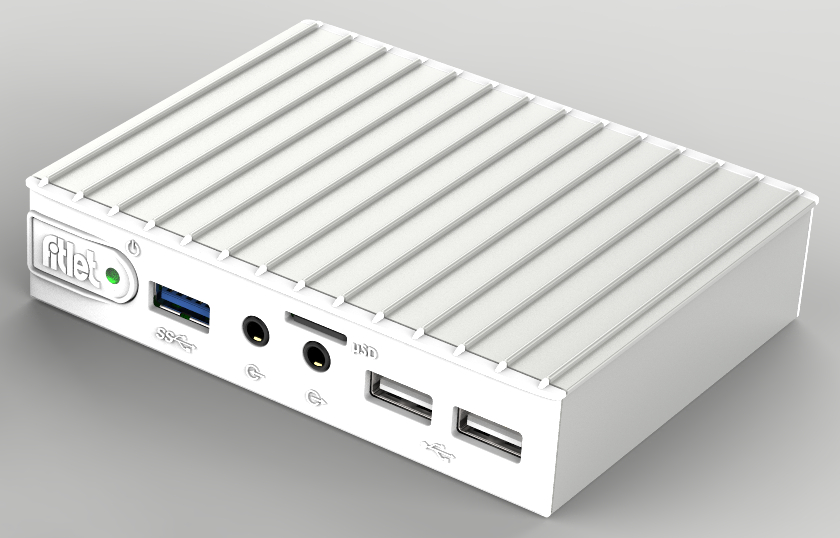
\includegraphics[width=0.5\linewidth]{../media/fitlet.jpg}
                    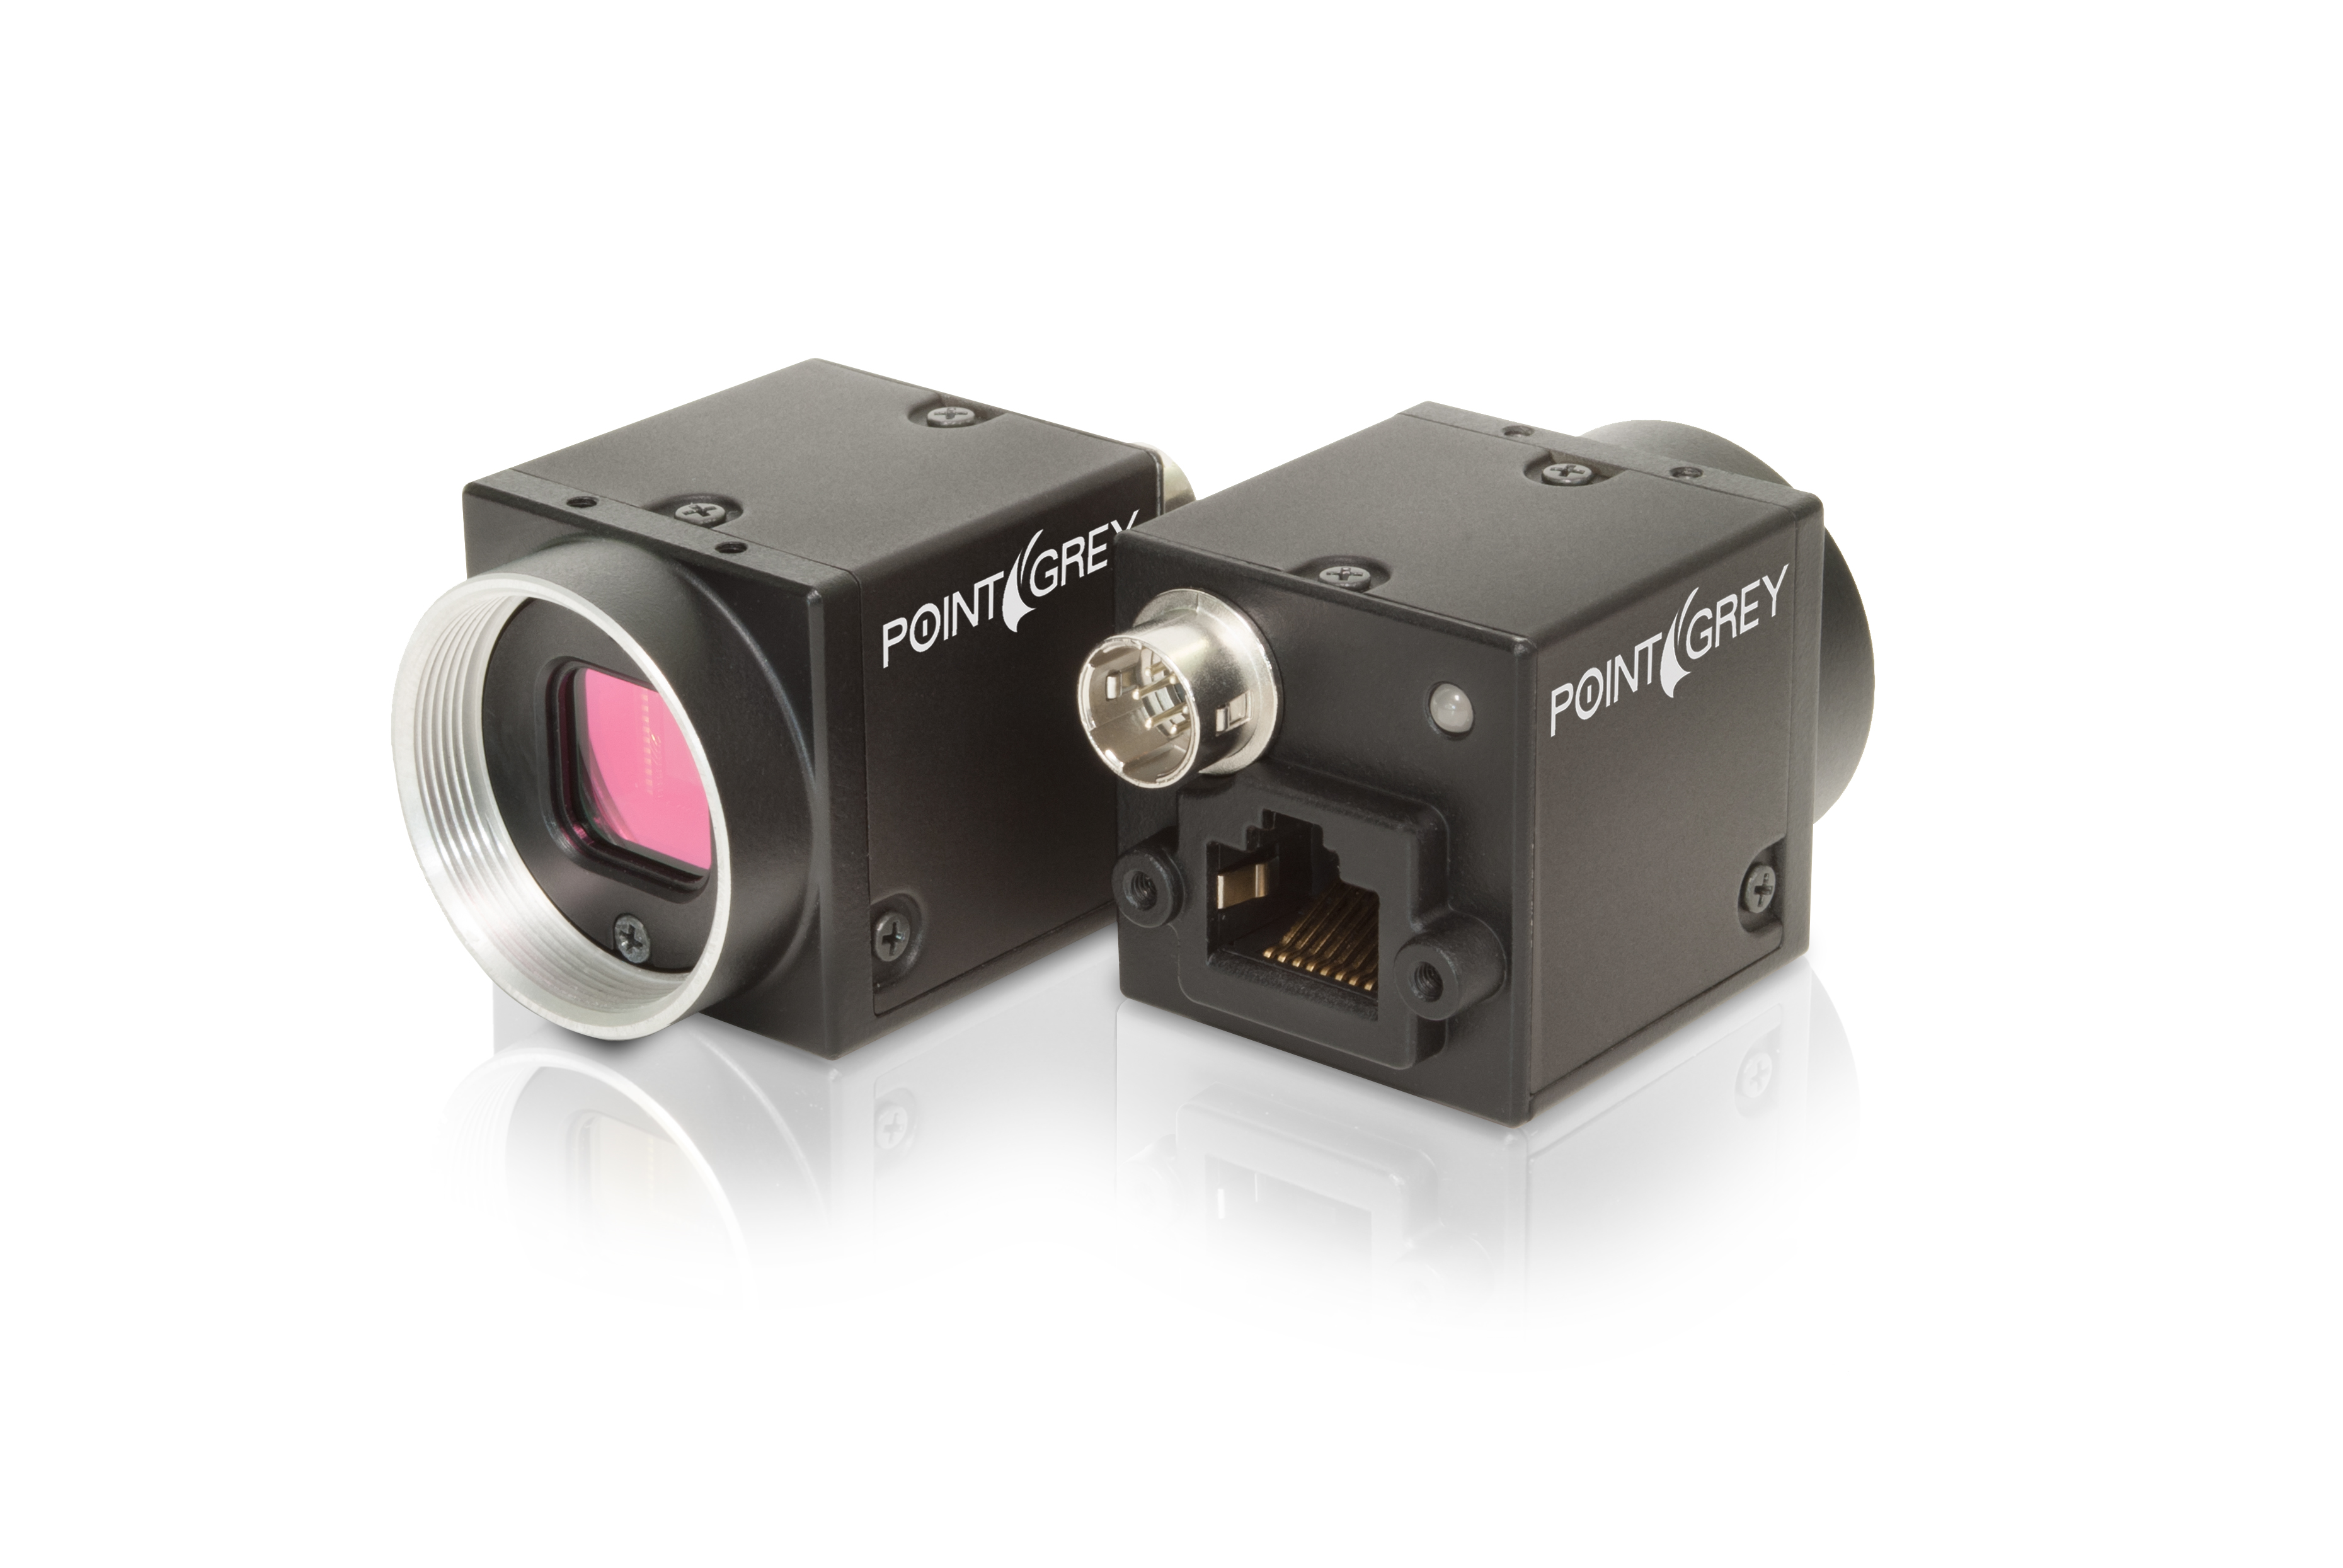
\includegraphics[width=0.6\linewidth]{../media/camera_blackfly.jpg}
                \end{column}
            \end{columns}
            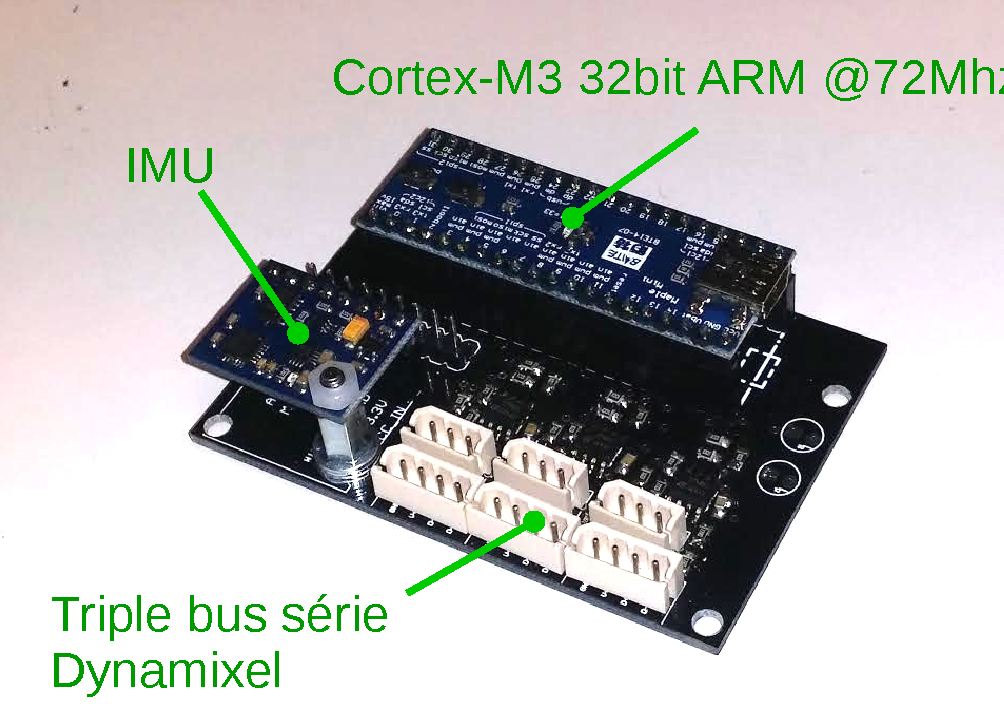
\includegraphics[type=pdf,ext=.pdf,read=.pdf,height=2cm]{../schema/3bus}
            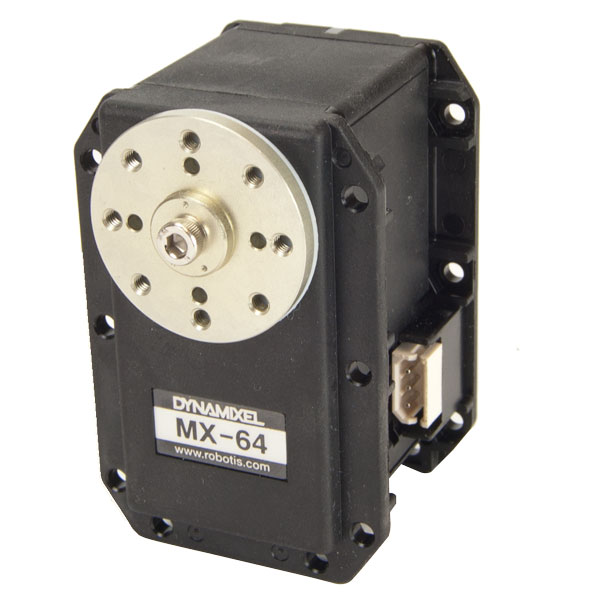
\includegraphics[height=2cm]{../media/dynamixel1.jpg}
            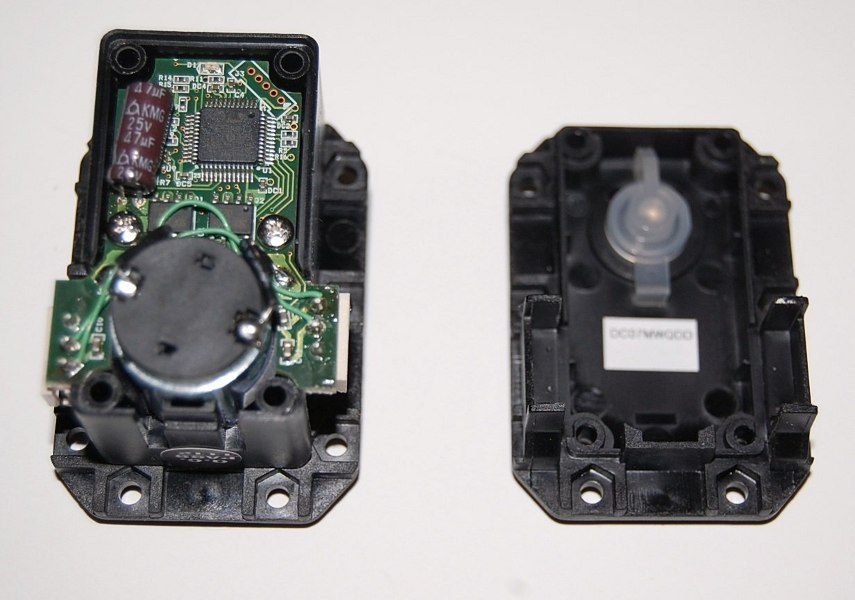
\includegraphics[height=2cm]{../media/dynamixel2.jpg}
        \end{column}
    \end{columns}
\end{frame}

\begin{frame}{Le robot Sigmaban (2/2) -- Robuste mais imparfait}
    \begin{columns}
        \begin{column}{0.55\linewidth}
            \begin{block}{Imperfections}
                Comportement réel $\neq$
                prédiction du modèle solide rigide
            \end{block}
            Robots humanoïdes précis :
            HRP-2, ASIMO, iCub (jambes), HOAP-3\\
            \vspace{1.0em}
            Nos robots :
            \begin{itemize}
                \item Coût moindre
                \item Nombreuses imperfections
                \item Matchs RoboCup : chocs importants, chutes fréquentes
                \item Robustes et solides
            \end{itemize}
        \end{column}
        \begin{column}{0.45\linewidth}
            \vspace{-1.2em}
            \begin{center}
            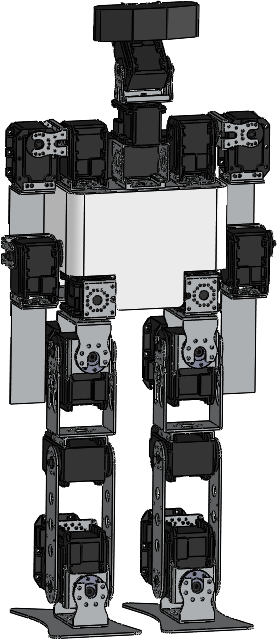
\includegraphics[height=2.9cm]{../media/sigmaban_cao2.png}
            \hspace{0.5cm}
            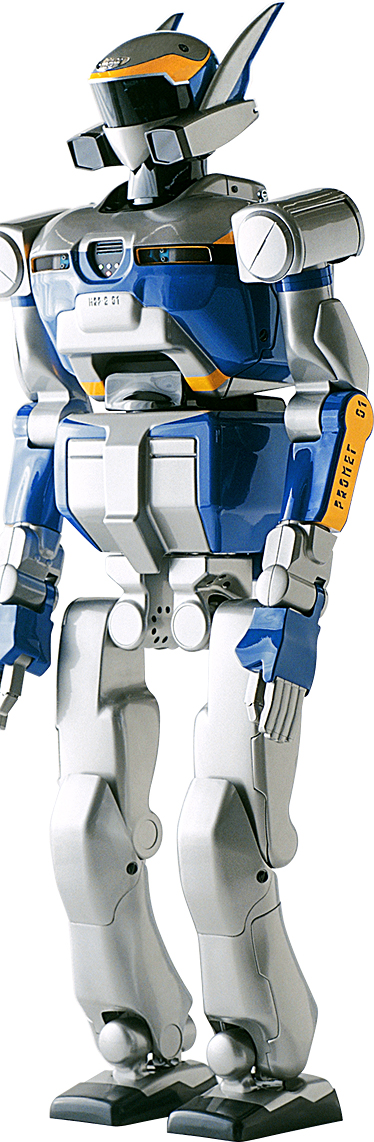
\includegraphics[height=8cm]{../media/hrp2.jpg}
            \newline
            \scriptsize
            (Source : Shuuji Kajita et al.)
            \end{center}
        \end{column}
    \end{columns}
\end{frame}

\begin{frame}{Imperfections (1/3) -- Déformations mécaniques}
    \begin{columns}
        \begin{column}{0.5\linewidth}
            \centering
            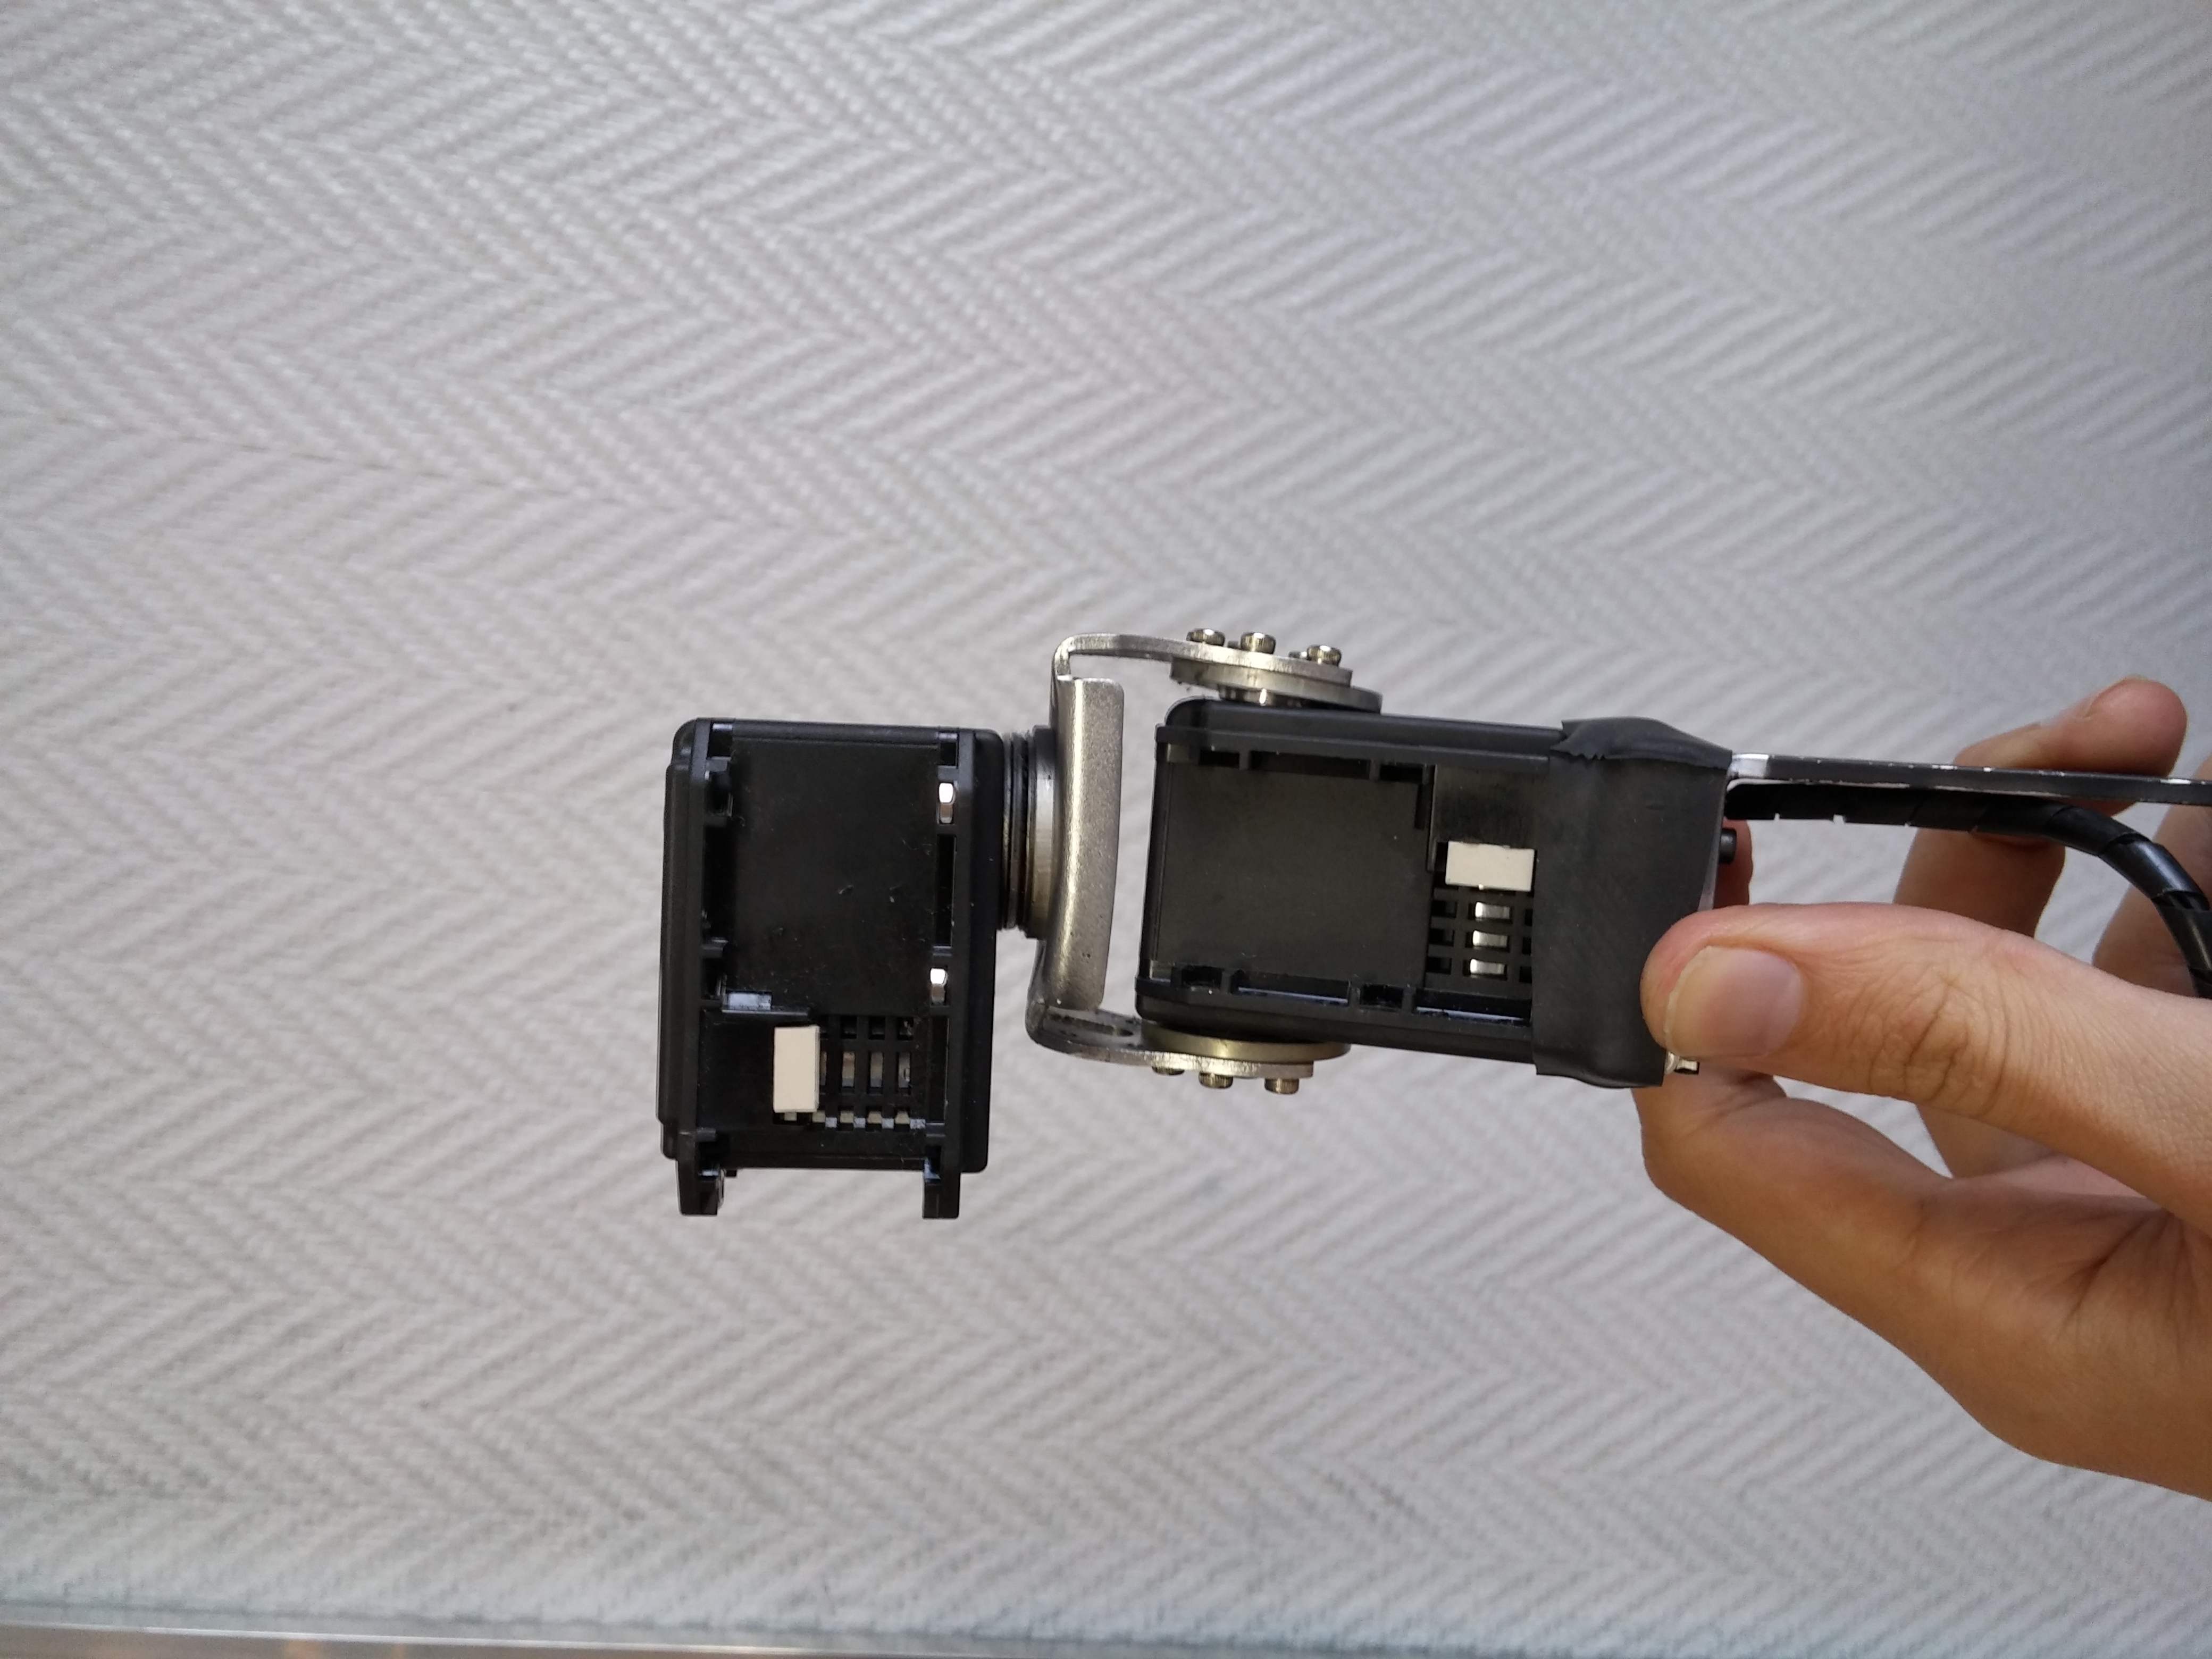
\includegraphics[height=4.5cm]{../media/torsion_meca1.jpg}
        \end{column}
        \begin{column}{0.5\linewidth}
            \centering
            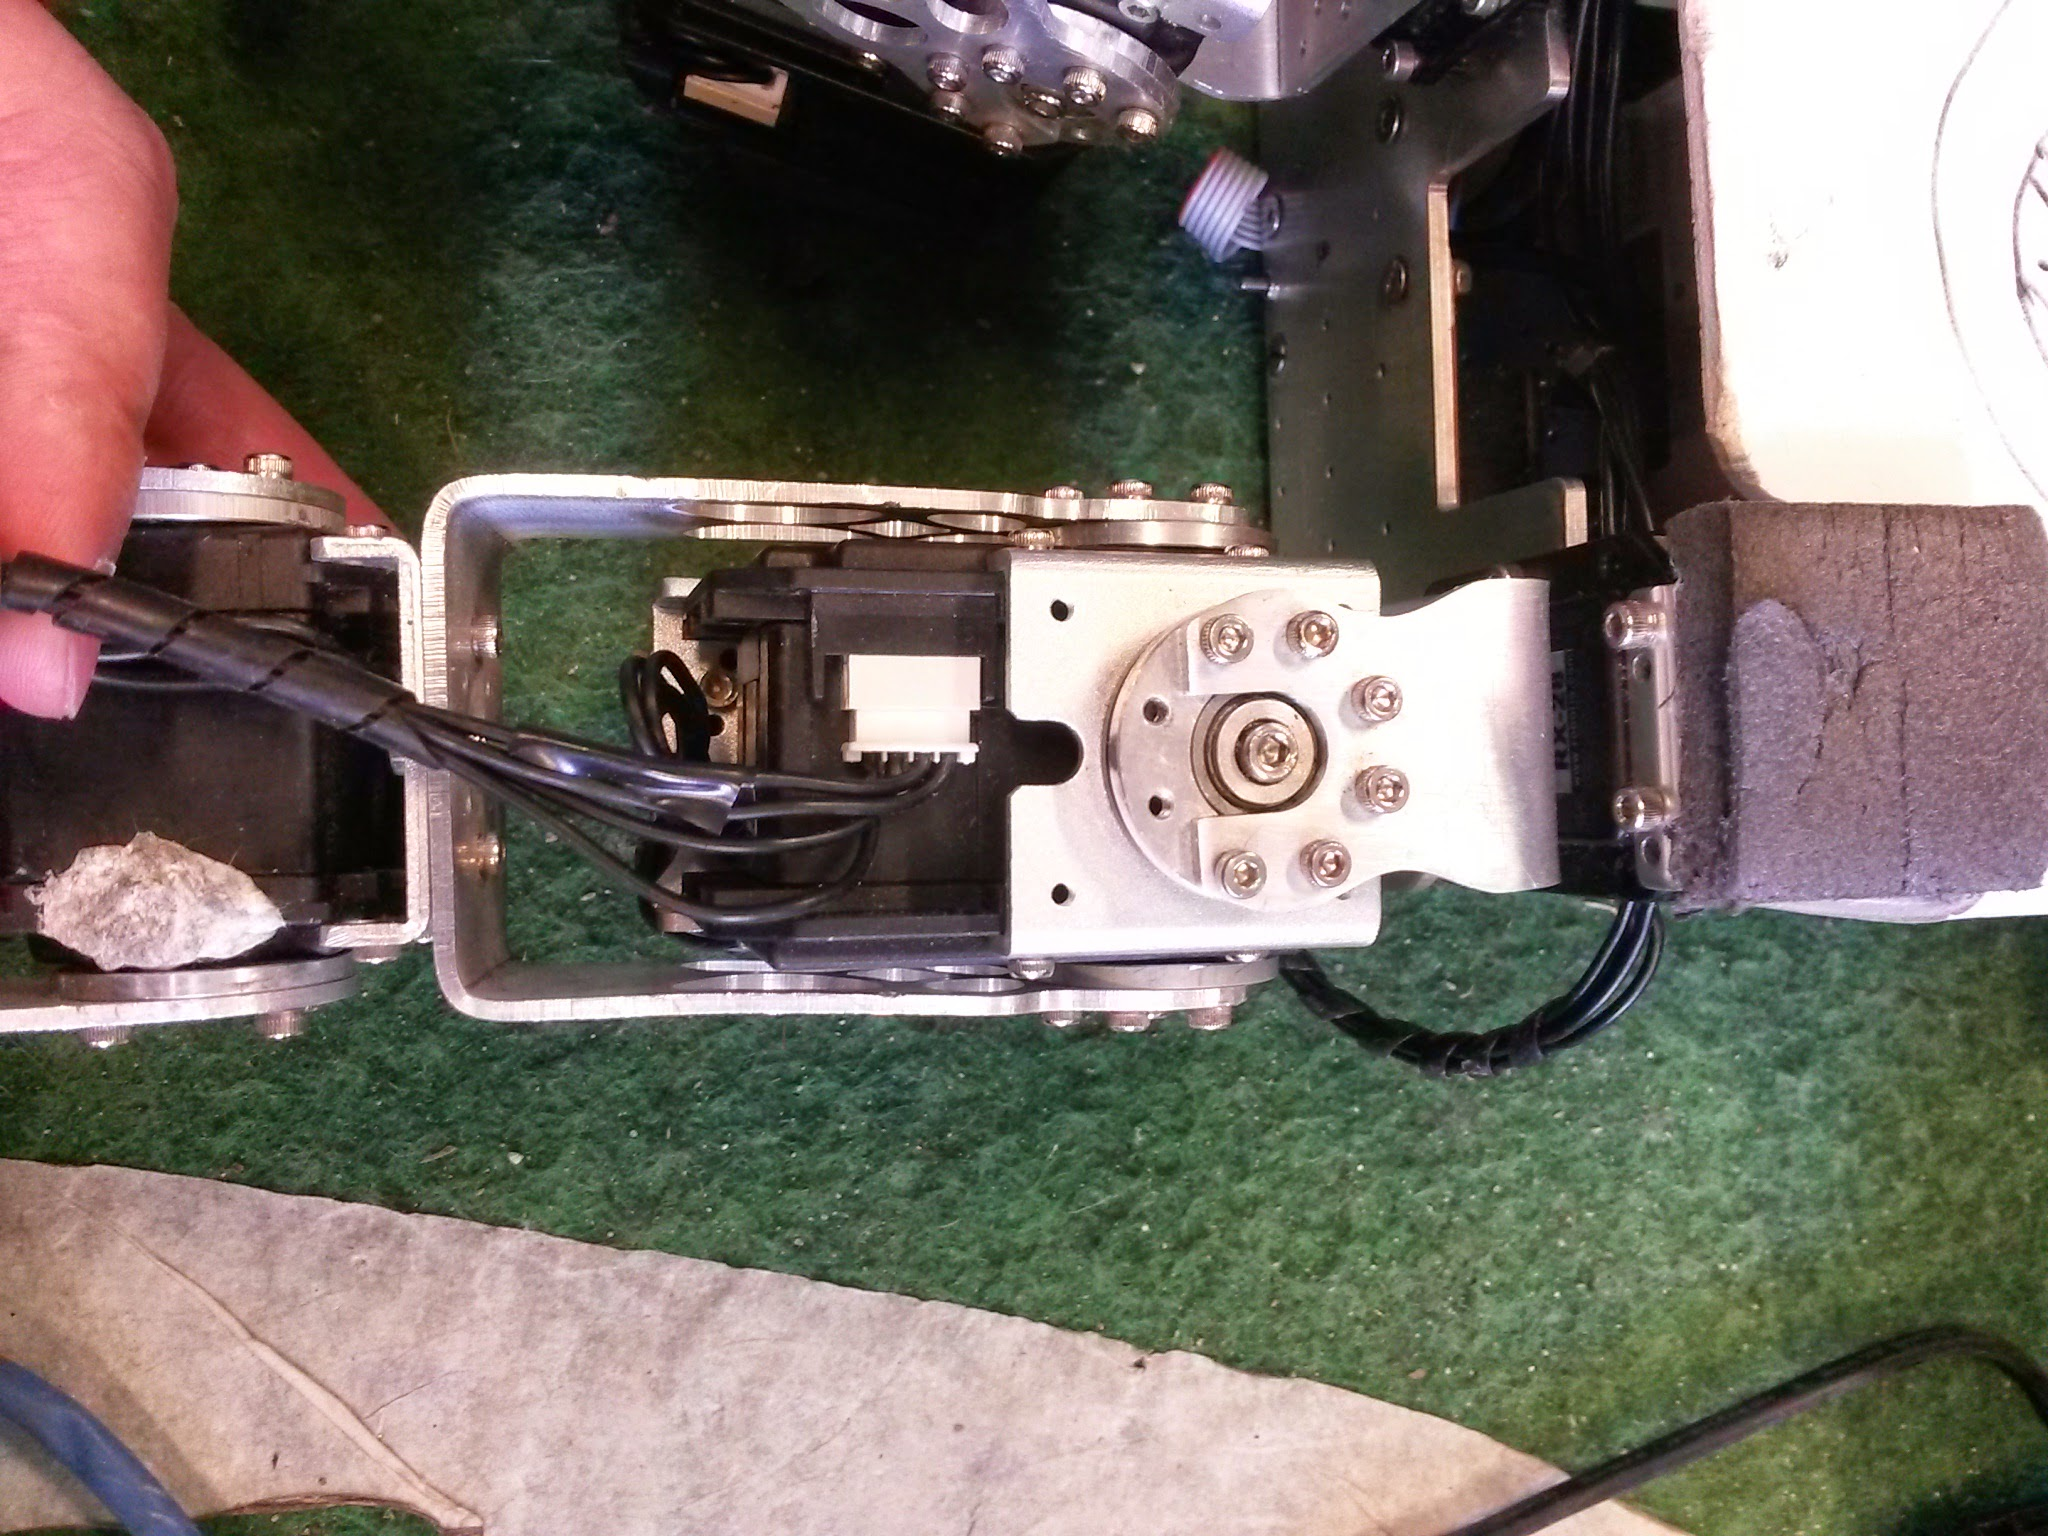
\includegraphics[height=4.5cm]{../media/torsion_meca2.jpg}
        \end{column}
    \end{columns}
    \vspace{1.0em}
    \begin{itemize}
        \item Segments mécaniques et torsions arbres moteur
        \item Usure : chutes et collisions
        \item Erreur statique du modèle géométrique
    \end{itemize}
\end{frame}

\begin{frame}{Imperfections (2/3) -- Jeu des engrenages}
    \begin{columns}
        \begin{column}{0.5\linewidth}
            \centering
            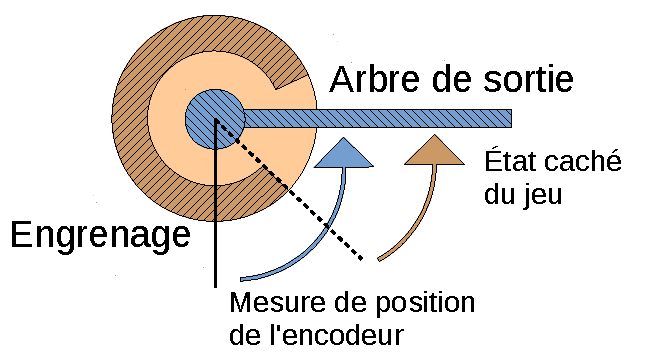
\includegraphics[type=pdf,ext=.pdf,read=.pdf,width=0.8\linewidth]{../schema/backlash_meca}
        \end{column}
        \begin{column}{0.5\linewidth}
            \centering
            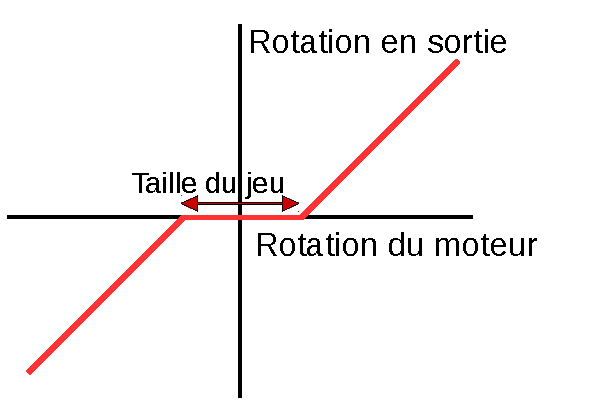
\includegraphics[type=pdf,ext=.pdf,read=.pdf,width=0.8\linewidth]{../schema/backlash_function}
        \end{column}
    \end{columns}
    \vspace{1.0em}
    \begin{itemize}
        \item Augmente avec l'âge du robot
        \item Mesuré par les encodeurs
        \item Affecte la dynamique
    \end{itemize}
\end{frame}

\begin{frame}{Imperfections (3/3) -- Asservissement des servomoteurs}
    \begin{columns}
        \begin{column}{0.5\linewidth}
            \begin{itemize}
                \item Asservissement réactif (proportionnel)
                \item Erreur angulaire > $10$\degres
            \end{itemize}
        \end{column}
        \begin{column}{0.5\linewidth}
            \centering
            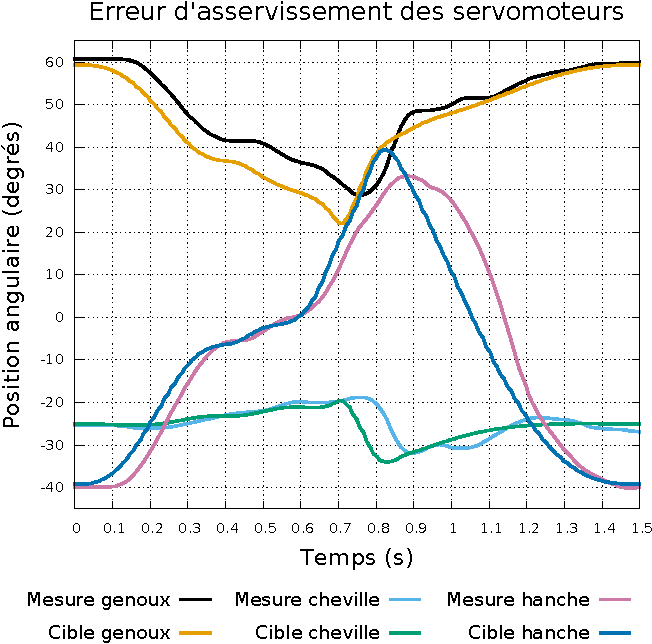
\includegraphics[type=pdf,ext=.pdf,read=.pdf,width=0.9\linewidth]{../plot/motors_control}
        \end{column}
    \end{columns}
    Pré-compensation (\textit{feedforward}) :
    \begin{block}{}
        \customtextcolor{
            \small
            \textit{Dynaban, an open-source alternative firmware for dynamixel servomotors}}\\
        \scriptsize
        Rémi Fabre, Quentin Rouxel, Grégoire Passault, Steve N'Guyen, Olivier Ly\\
        Symposium RoboCup, 2016\\
    \end{block}
    $\Rightarrow$ Pas utilisé dans la suite
\end{frame}



\subsection{Problématique}

\begin{frame}{Problématique scientifique}
    \begin{columns}
        \begin{column}{0.56\linewidth}
            \begin{description}
                \setlength\itemsep{1em}
                \item[Difficultés]
                    \begin{itemize}
                        \item Petits robots humanoïdes
                        \item Nombreuses imperfections
                    \end{itemize}
                \item[Problème] 
                    \begin{itemize}
                        \item Réduire écart comportement estimé/désiré et réalité
                        \item Méthodes d'apprentissage
                    \end{itemize}
                \item[Applications] Compétition RoboCup
                    \begin{itemize}
                        \item Déplacement du robot (odométrie)
                        \item Modèle de caméra
                        \item Synthèse de mouvements dynamiques
                    \end{itemize}
                \item[Contexte]
                    \begin{itemize}
                        \item Puissance de calcul limité (autonomie)
                        \item Solutions opérationnelles
                    \end{itemize}
            \end{description}
        \end{column}
        \begin{column}{0.44\linewidth}
            \centering
            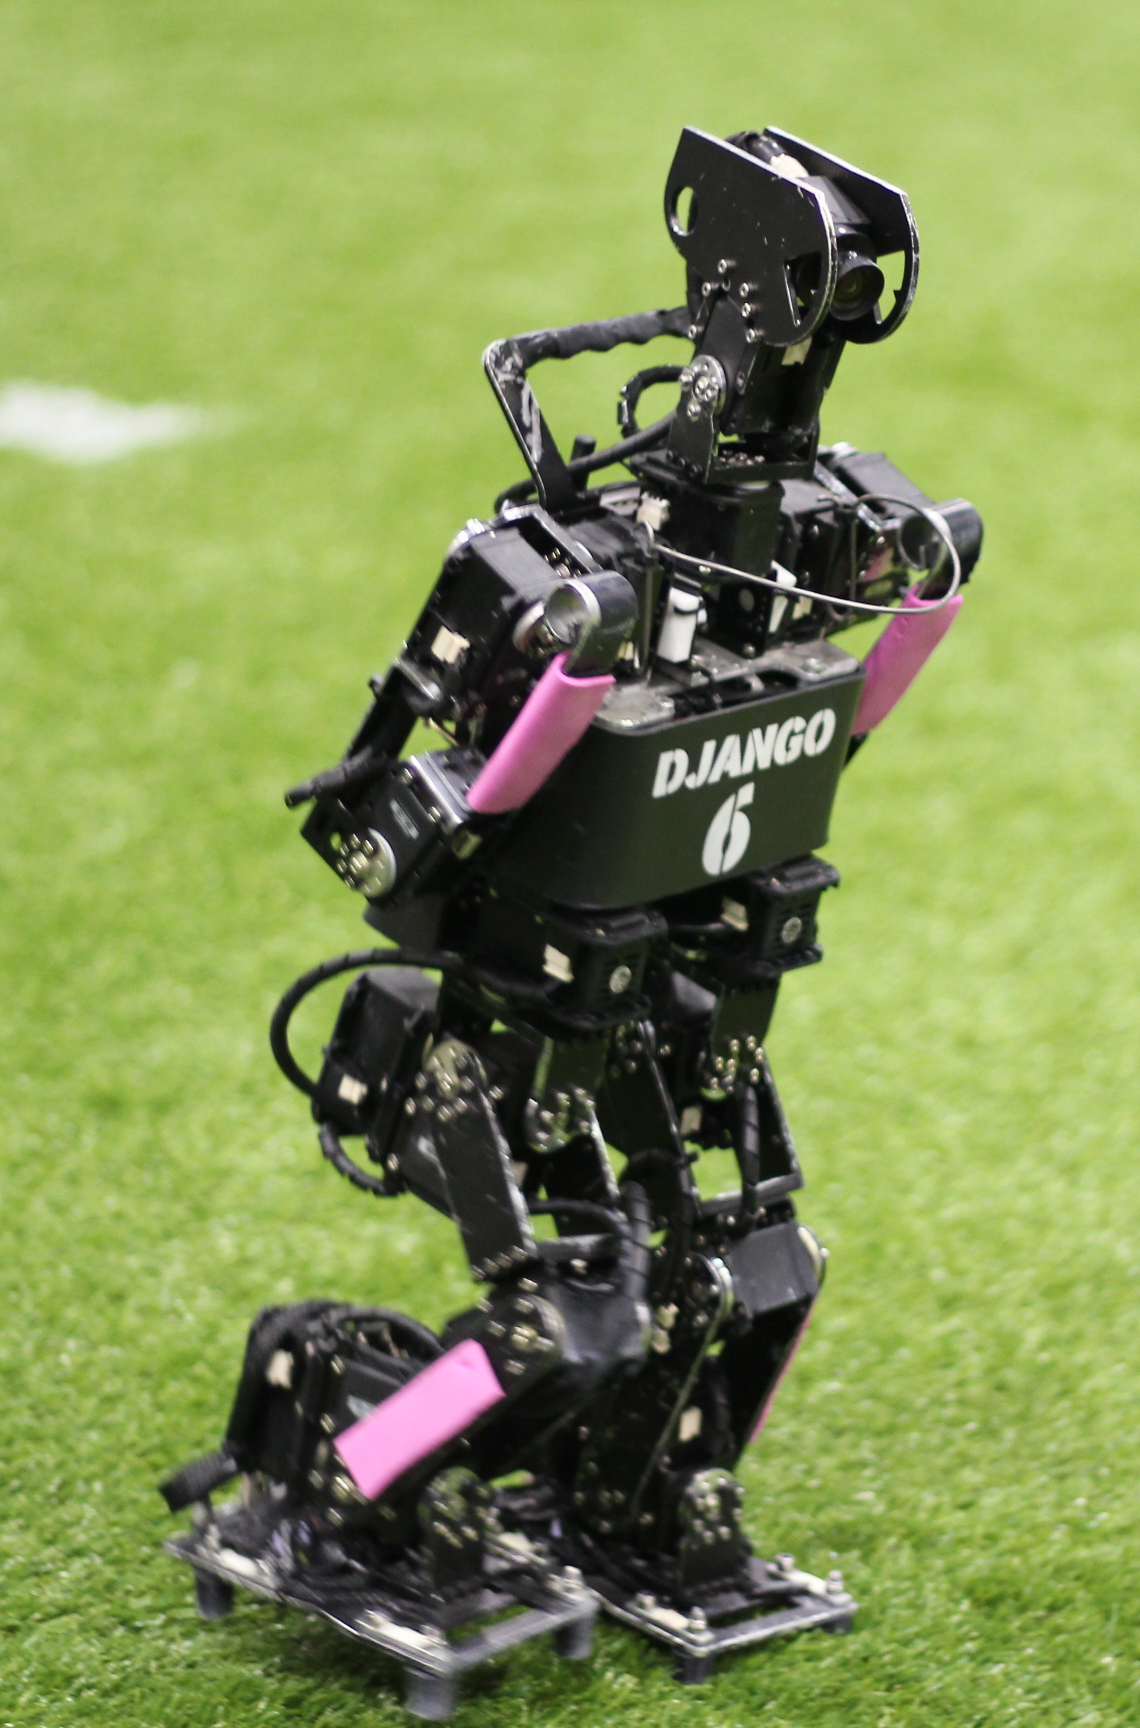
\includegraphics[height=4.0cm]{../media/sigmaban_1_6.png}
            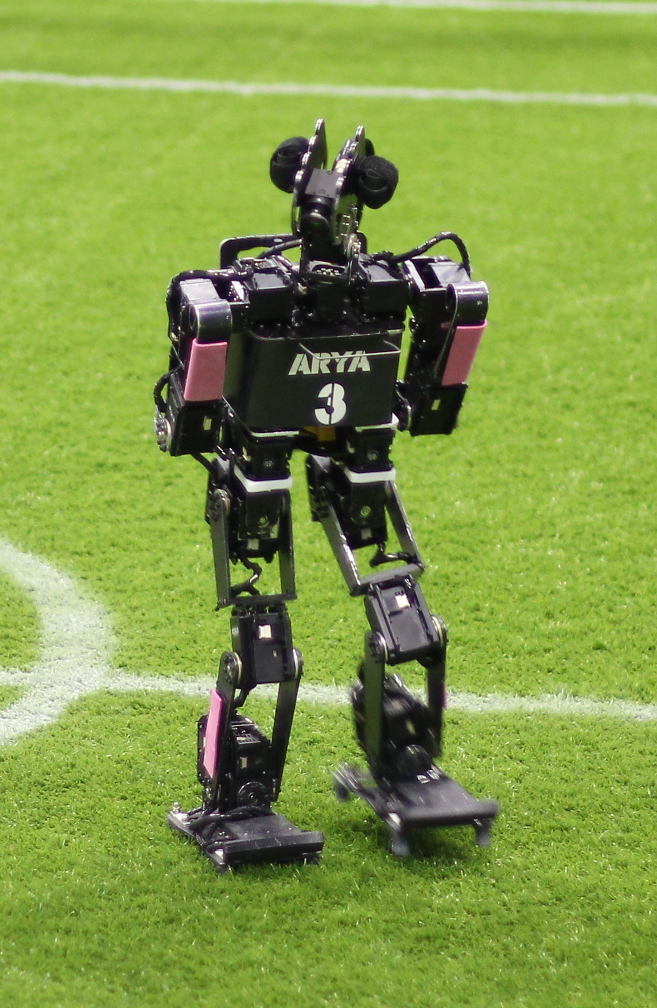
\includegraphics[height=4.0cm]{../media/grosban_1_2.png}
        \end{column}
    \end{columns}
\end{frame}



\section{Définitions et notions}

\begin{frame}{Définitions et notions}
    \tableofcontents[ 
        sectionstyle=show/shaded, 
        subsectionstyle=show/shaded, 
        currentsubsection, 
        hideothersubsections, 
    ] 
\end{frame}


\subsection{Définitions}

\begin{frame}{Définitions (1/2) -- Déplacement égocentrique}
    \begin{columns}
        \begin{column}{0.49\textwidth}
            \begin{block}{Repère égocentrique}
                Projection du repère du buste
            \end{block}
            \begin{block}{Pose}
                Position + orientation $\in \mathbb{R}^2 \times ]-\pi,\pi]$
            \end{block}
            \begin{block}{Pied de support}
                Pied en contact avec le sol
            \end{block}
            \begin{block}{Déplacement égocentrique}
                Variation de la pose du repère égocentrique
                entre deux changements de pied de support
                $
                \Delta \bm{p} =
                \begin{bmatrix}
                    \Delta x \\ \Delta y \\ \Delta \theta 
                \end{bmatrix}
                \in \mathbb{R}^3
                $
            \end{block}
        \end{column}
        \begin{column}{0.49\textwidth}
            \centering
            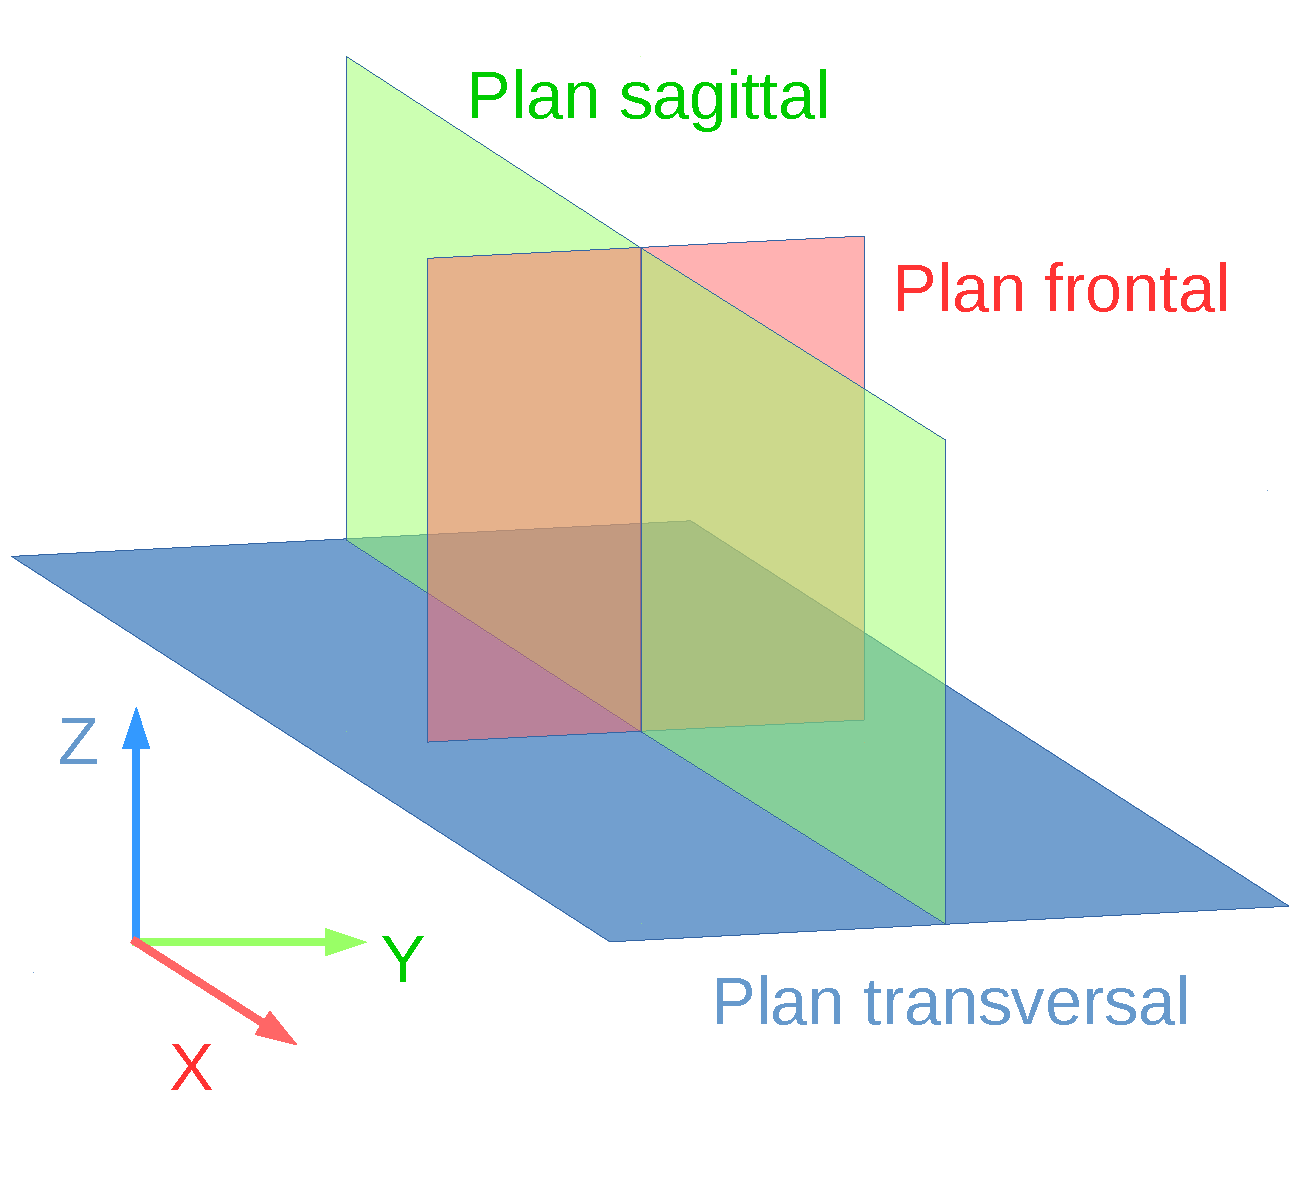
\includegraphics[type=pdf,ext=.pdf,read=.pdf,width=0.6\linewidth]{../schema/planes}
            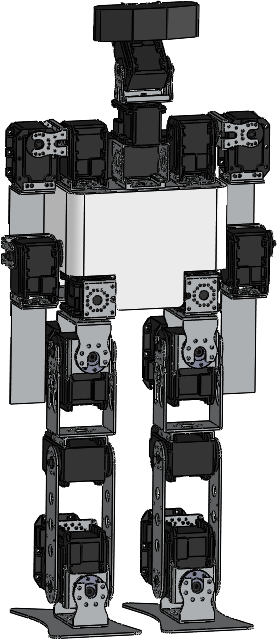
\includegraphics[width=0.25\linewidth]{../media/sigmaban_cao2.png}
            \newline
            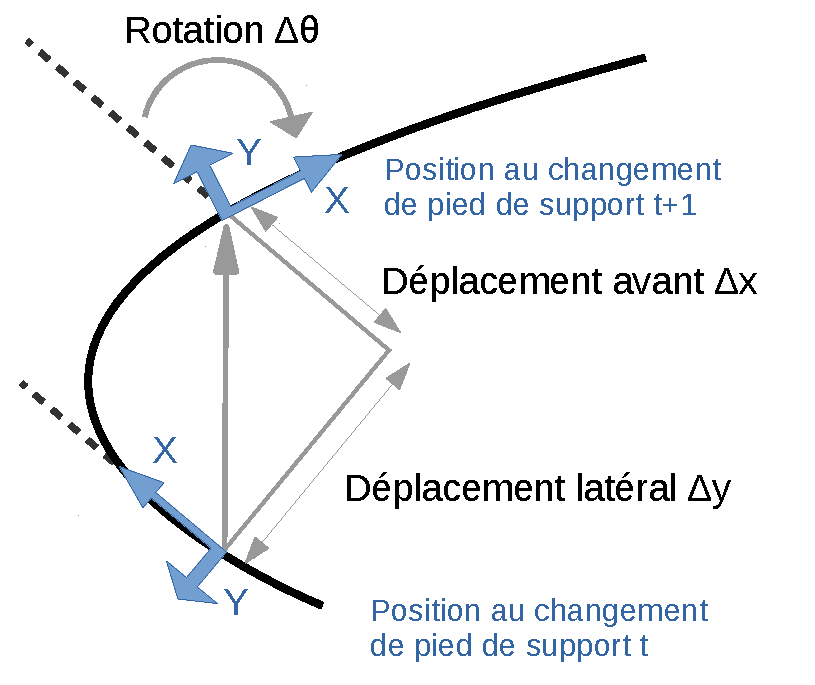
\includegraphics[type=pdf,ext=.pdf,read=.pdf,width=0.9\linewidth]{../schema/footstep}
        \end{column}
    \end{columns}
\end{frame}

\begin{frame}{Définitions (2/2) -- Odométrie proprioceptive et prédictive}
    \begin{block}{Odométrie proprioceptive}
        \begin{columns}
            \begin{column}{0.4\textwidth}
                Capteurs proprioceptifs
                (encodeurs, IMU, pression)
            \end{column}
            \begin{column}{0.2\textwidth}
                $\longmapsto$
            \end{column}
            \begin{column}{0.3\textwidth}
                Déplacements égocentriques
            \end{column}
        \end{columns}
    \end{block}
    \begin{block}{Odométrie prédictive (modèle de déplacement)}
        \begin{columns}
            \begin{column}{0.4\textwidth}
                Ordres de la marche
            \end{column}
            \begin{column}{0.2\textwidth}
                $\longmapsto$
            \end{column}
            \begin{column}{0.3\textwidth}
                Déplacements égocentriques
            \end{column}
        \end{columns}
    \end{block}
    \vspace{2.0em}
    \begin{itemize}
        \item Pas de caméra
        \item Précision odométrie proprioceptive > prédictive
        \item Apprentissage avec les mêmes données
        \item Intégration $\Rightarrow$ trajectoire
    \end{itemize}
\end{frame}

\subsection{Enjeux}

\begin{frame}{Applications pour la RoboCup}
    \begin{columns}
        \begin{column}{0.49\linewidth}
            Odométrie proprioceptive :
            \begin{itemize}
                \item Localisation
                \item Asservissement du déplacement
                \item Suivi de la balle
            \end{itemize}
        \end{column}
        \begin{column}{0.49\linewidth}
            Odométrie prédictive :
            \begin{itemize}
                \item Simulation du déplacement
                \item Tests comportements haut niveau
                \item Plannification de trajectoire
            \end{itemize}
        \end{column}
    \end{columns}
    \vspace{0.2cm}
    \centering
    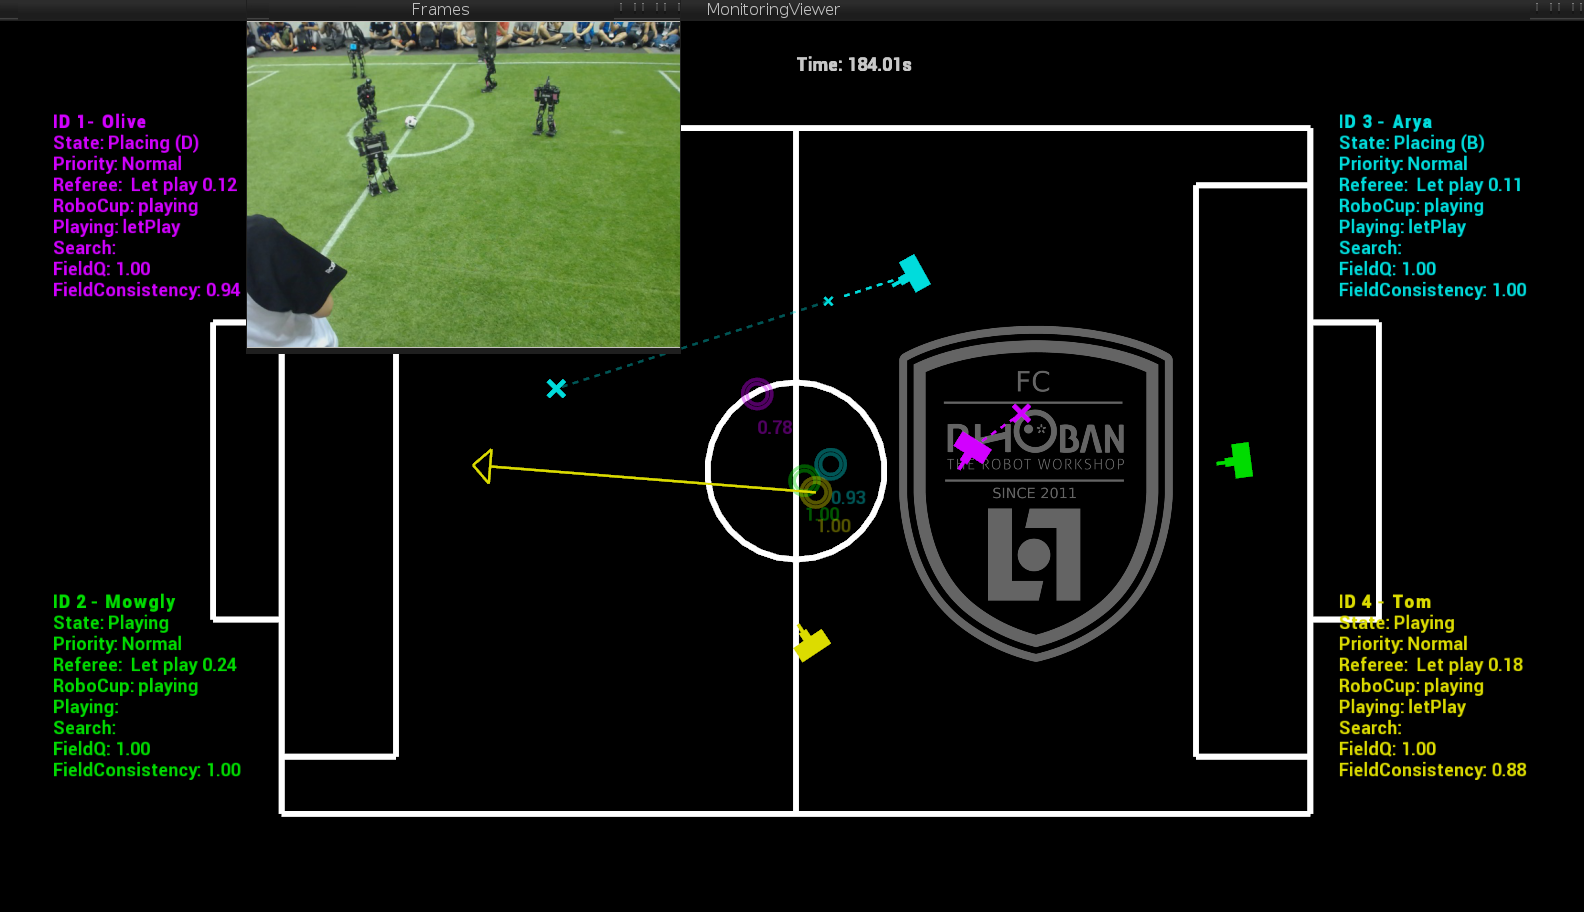
\includegraphics[width=0.85\linewidth]{../media/monitoring.png}
\end{frame}



\subsection{Littérature et état de l'art}

\begin{frame}{État de l'art (1/2) -- Apprentissage de l'odométrie}
    \footnotesize
    Littérature :
    \vspace{0.5em}
    \newline
    \begin{tabular}{|p{1.5cm}|l|p{1.7cm}|p{1.2cm}|p{1.8cm}|p{1.6cm}|}
        \hline
        Article & Robot & Mesure & Capteur & Apprentissage & Particularité \\
        \hline
        \customtextcolor{(Borenstein et al., 1996)} 
            & roues & trajectoires références & manuel & analytique & Benchmark \\
        \hline
        \customtextcolor{(Roy et al., 1999)} 
            & roues & déplacements égocentriques & laser proprioceptif & maximisation vraisemblance & \\
        \hline
        \customtextcolor{(Martínez et al., 2005)}
            & roues & pose finale & manuel & optimisation boite noire & chenilles \\
        \hline
        \customtextcolor{(Antonelli et al., 2005)}
            & roues & pose finale & externe & régression linéaire & linéarisation \\
        \hline
        \customtextcolor{(Schmitz et al., 2010)} 
            & humanoïde & déplacements égocentriques & externe & régression linéaire & uniquement prédiction \\
        \hline
    \end{tabular}
    \vspace{0.5em}
    \newline
    Contributions :
    \vspace{0.5em}
    \newline
    \begin{tabular}{|p{1.5cm}|l|p{1.7cm}|p{1.2cm}|p{1.8cm}|p{1.6cm}|}
        \hline
        \customtextcolor{(Rouxel et al., 2016)} 
            & humanoïde & déplacements égocentriques & externe & régression non paramétrique & proprioceptif + prédictif \\
        \hline
        \customtextcolor{(Hofer et al., 2017)} 
            & humanoïde & pose finale & manuel & optimisation boite noire & proprioceptif + prédictif \\
        \hline
    \end{tabular}
\end{frame}

\begin{frame}{État de l'art (2/2) -- Odométrie visuelle}
    \begin{block}{Odométrie visuelle}
        \begin{itemize}
            \item Traitement d'images
            \item Variation de la pose de la caméra entre deux images
            \item Dans le repère du monde
            \item Pas de proprioception
        \end{itemize}
    \end{block}
    \customtextcolor{Avantage :}\\
    ~~~prend en compte les glissements\\
    \customtextcolor{Principales difficultés :}\\
    ~~~puissance de calcul, chocs et mouvements saccadés $\Rightarrow$ flou et bruit\\
    \vspace{1.0em}
    \begin{description}
        \item[Stasse et al. (2006)] : 
            robot humanoïde HRP-2 + déplacement désiré + Kalman
        \item[Oriolo et al. (2016)] : 
            robot NAO + odométrie prorioceptive + capteur FSR + Kalman (mais calcul déporté)
    \end{description}
\end{frame}


%
\begin{frame}[noframenumbering]{Mouvement de marche}
    \begin{columns}
        \begin{column}{0.4\textwidth}
            \begin{itemize}
                \item Générateur \textit{IKWalk} boucle ouverte + stabilisation
                \item Holonome
                \item Réglage manuel par expérimentation
                \item Mouvement désiré $\neq$ mesuré
                \item Amélioration 2017 : générateur \textit{QuinticWalk}
            \end{itemize}
        \end{column}
        \begin{column}{0.6\textwidth}
            \centering
            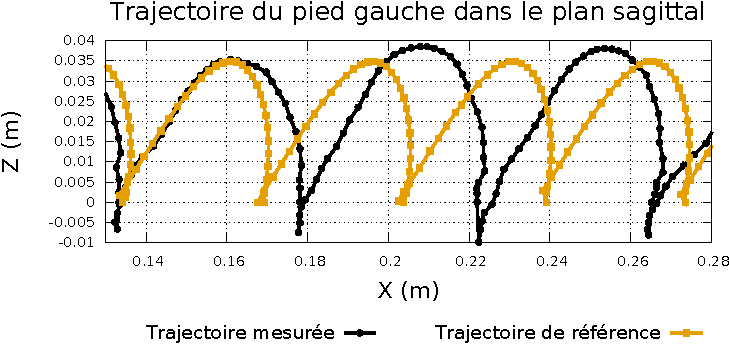
\includegraphics[type=pdf,ext=.pdf,read=.pdf,width=1.0\linewidth]{../plot/walk_traj_foot}
        \end{column}
    \end{columns}
    \vspace{0.2cm}
    \begin{block}{}
        \customtextcolor{
            \small
            \textit{Rhoban hardware and software open source contributions for robocup humanoids}}\\
        \scriptsize
        Quentin Rouxel, Grégoire Passault, Ludovic Hofer, Steve N'Guyen, Olivier Ly\\
        Workshop on Humanoid Soccer Robots, 2015\\
    \end{block}
\end{frame}

\begin{frame}[noframenumbering]{Mouvement de marche (2/3) -- Générateur \textit{IKWalk}}
    \centering
    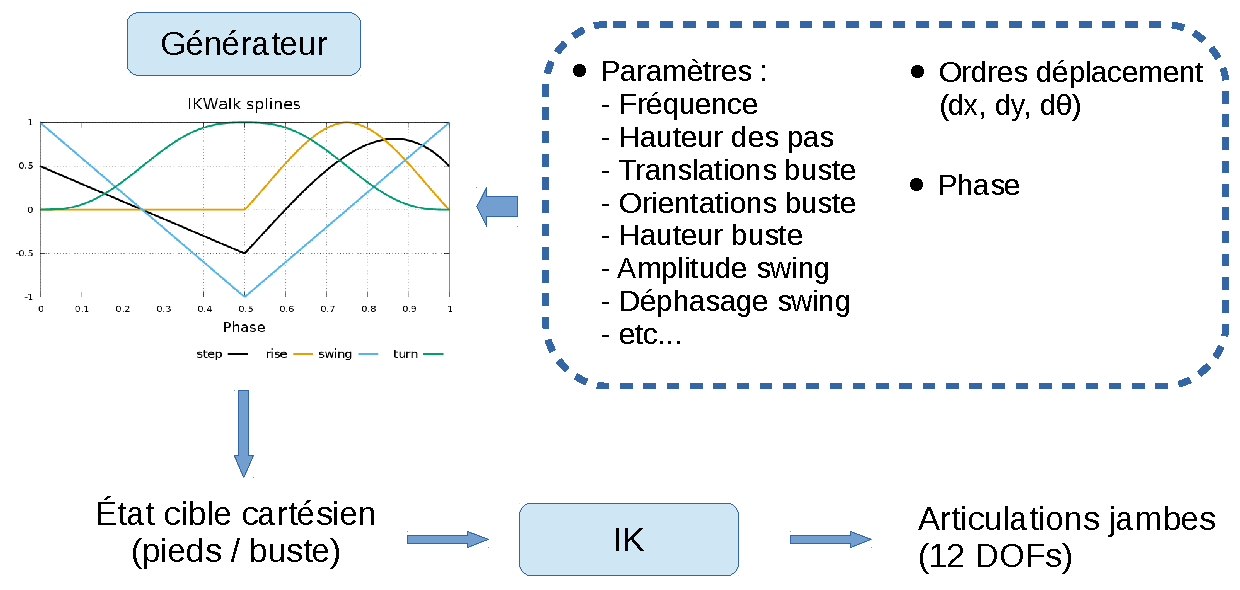
\includegraphics[type=pdf,ext=.pdf,read=.pdf,width=1.0\linewidth]{../schema/ikwalk}
    \begin{block}{}
        \customtextcolor{
            \small
            \textit{Rhoban hardware and software open source contributions for robocup humanoids}}\\
        \scriptsize
        Quentin Rouxel, Grégoire Passault, Ludovic Hofer, Steve N'Guyen, Olivier Ly\\
        Workshop on Humanoid Soccer Robots, 2015\\
    \end{block}
\end{frame}

\begin{frame}[noframenumbering]{Mouvement de marche (3/3) -- Stabilisation}
    \begin{columns}
        \begin{column}{0.5\textwidth}
            \begin{itemize}
                \item Stabilisation latérale
                \item Position du centre de pression
                \item Mise en pause du mouvement
            \end{itemize}
        \end{column}
        \begin{column}{0.5\textwidth}
            \centering
            \movie[
                autostart,
                width=\linewidth, 
                height=0.56\linewidth,
                poster,
                loop
            ]{}{../video/cutStabilization_light.mp4}
            \scriptsize
            (Source : Grégoire Passault)
        \end{column}
    \end{columns}
    \centering
    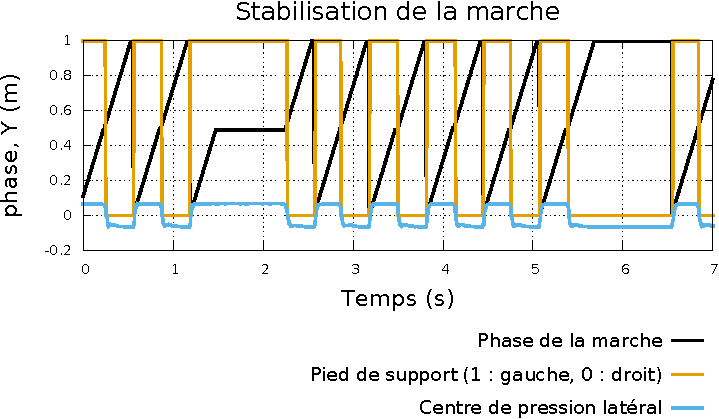
\includegraphics[type=pdf,ext=.pdf,read=.pdf,width=0.6\linewidth]{../plot/walk_stabilization1}
\end{frame}


\subsection{Proprioception}

\begin{frame}{Estimation de l'odométrie (1/3) -- Modèle géométrique}
    \begin{columns}
        \begin{column}{0.45\linewidth}
            Humanoïdes $\Rightarrow$ déplacement \og sous actué \fg\\
            \vspace{1.0em}
            \begin{block}{Modèle géométrique direct}
                espace articulaire (moteurs) $\longmapsto$ espace cartésien (monde 3D)
            \end{block}
            \vspace{1.0em}
            Hypothèses :
            \begin{itemize}
                \item Pas de glissement
                \item Toujours un pied au sol
                \item Pas de double support
                \item Pied de support non posé à plat
            \end{itemize}
        \end{column}
        \begin{column}{0.55\linewidth}
            \centering
            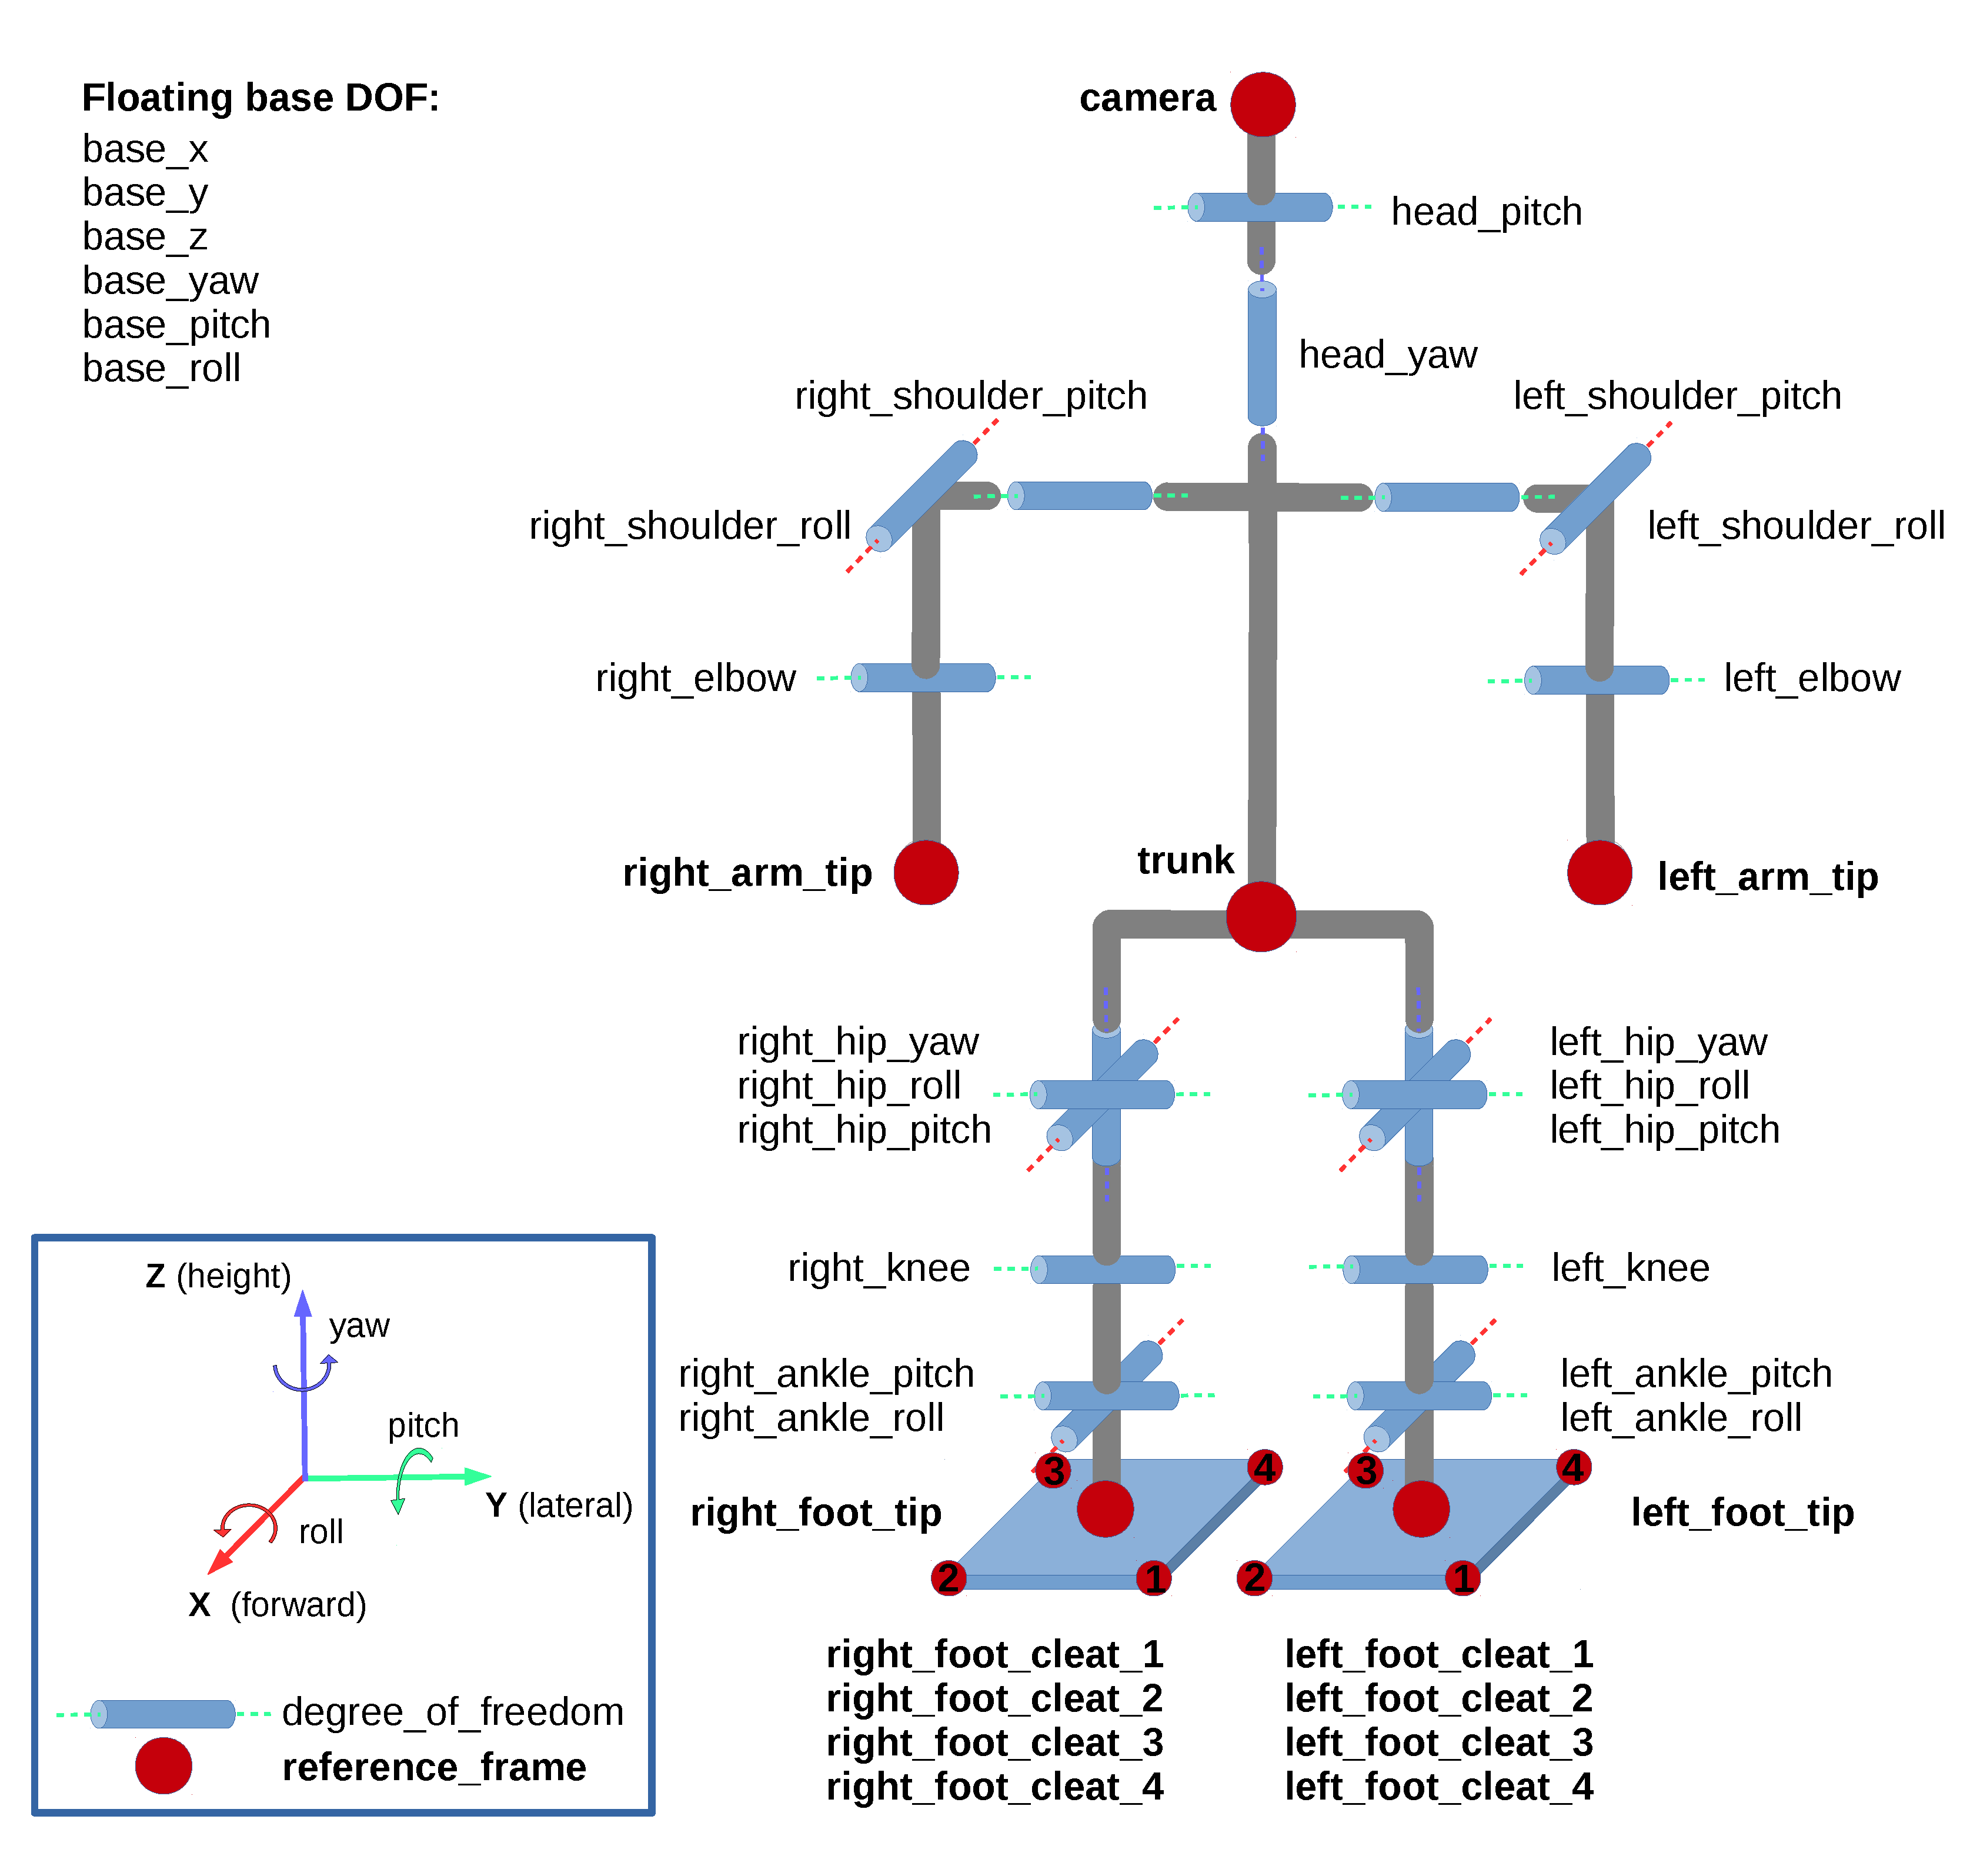
\includegraphics[type=pdf,ext=.pdf,read=.pdf,width=1.0\linewidth]{../schema/humanoid}
        \end{column}
    \end{columns}
\end{frame}

\begin{frame}{Estimation de l'odométrie (2/3) -- Proprioception}
    \begin{columns}
        \begin{column}{0.5\linewidth}
            Capteurs :
            \begin{itemize}
                \item Estimation du pied de support
                \item Encodeurs $\Rightarrow$ angles articulations
                \item Centrale inertielle (IMU) :
                    \begin{itemize}
                        \item accéléromètres, gyromètres
                        \item filtrage de Mahony
                        \item inclinaison du buste
                    \end{itemize}
                \item Intégration des gyromètres $\Rightarrow$ azimut du buste
            \end{itemize}
        \end{column}
        \begin{column}{0.5\linewidth}
            \centering
            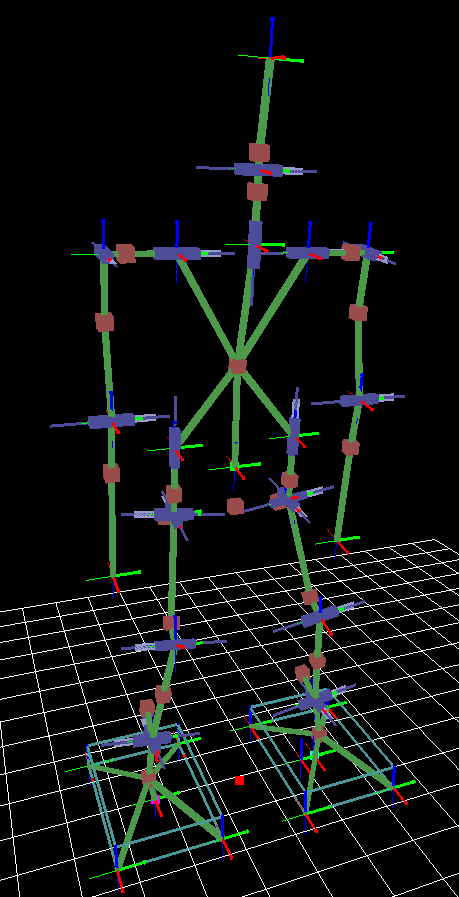
\includegraphics[height=0.85\textheight]{../media/model_gui1.png}
        \end{column}
    \end{columns}
\end{frame}

\begin{frame}{Estimation de l'odométrie (3/3) -- Intégration}
    \begin{columns}
        \begin{column}{0.5\linewidth}
            Odométrie proprioceptive :
            \begin{itemize}
                \item Capteurs $\Rightarrow$ état géométrique
                \item Au changement de pied de support :
                    \begin{itemize}
                        \item Calcul de la pose du deuxième pied
                        \item Changement et conversion du modèle géométrique (autre pied)
                    \end{itemize}
            \end{itemize}
            \vspace{1.0em}
            Odométrie prédictive :
            \begin{itemize}
                \item Ordres de déplacement $\Rightarrow$ générateur de marche $\Rightarrow$
                    positions articulaires désirées
                \item Pied à plat sur le sol
                \item Pied de support imposé par la marche
            \end{itemize}
        \end{column}
        \begin{column}{0.5\linewidth}
            \centering
            \movie[
                autostart,
                width=\linewidth, 
                height=0.76\linewidth,
                poster,
                loop
            ]{}{../video/walk.ogv}
        \end{column}
    \end{columns}
\end{frame}



\subsection{Pied de support}

\begin{frame}{Proprioception du pied de support (1/2) -- Méthodes}
    \begin{columns}
        \begin{column}{0.4\linewidth}
            \begin{block}{Estimation par le modèle géométrique}
                Pied le plus bas
            \end{block}
            \begin{block}{Estimation par les capteurs de pression}
                Pied mesurant le plus de poids
            \end{block}
            \vspace{1.0em}
            \centering
            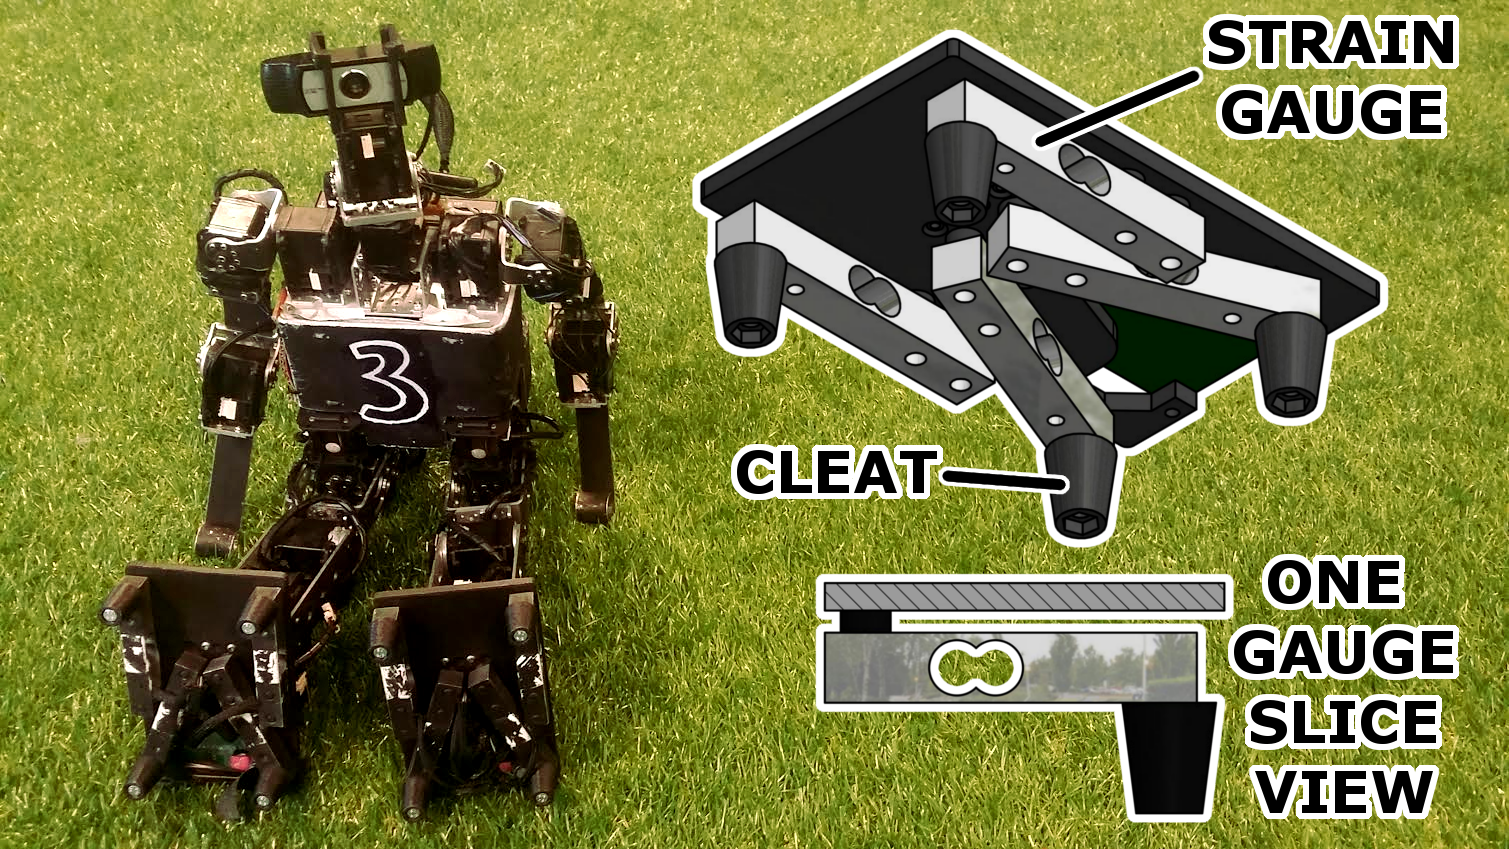
\includegraphics[width=1.0\linewidth]{../media/pressures1.png}
        \end{column}
        \begin{column}{0.6\linewidth}
            \centering
            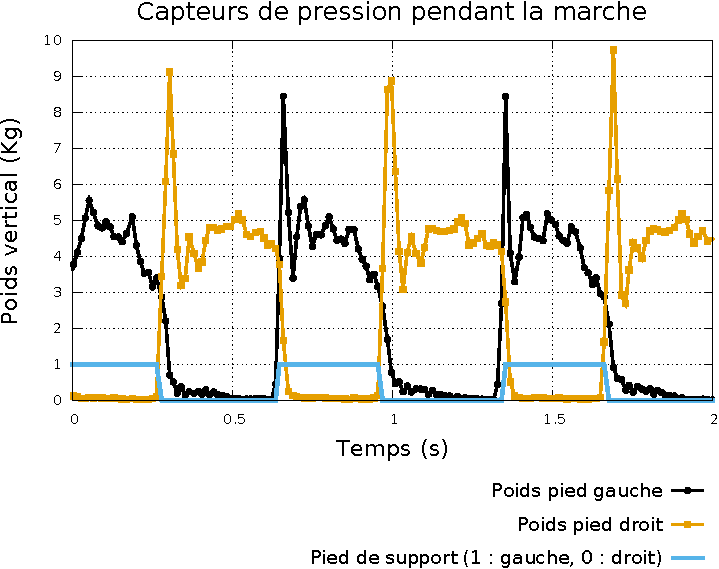
\includegraphics[type=pdf,ext=.pdf,read=.pdf,width=1.0\linewidth]{../plot/pressure_sensors}
        \end{column}
    \end{columns}
\end{frame}

\begin{frame}{Proprioception du pied de support (2/2) -- Comparaison}
    \begin{columns}
        \begin{column}{0.4\linewidth}
            Pilotage manuel. Comparaison de l'odométrie proprioceptive :
            \vspace{1.0em}
            \begin{itemize}
                \setlength\itemsep{1em}
                \item Capteurs de pression > modèle géométrique directe
                \item Dérive de l'azimut
            \end{itemize}
        \end{column}
        \begin{column}{0.6\linewidth}
            \centering
            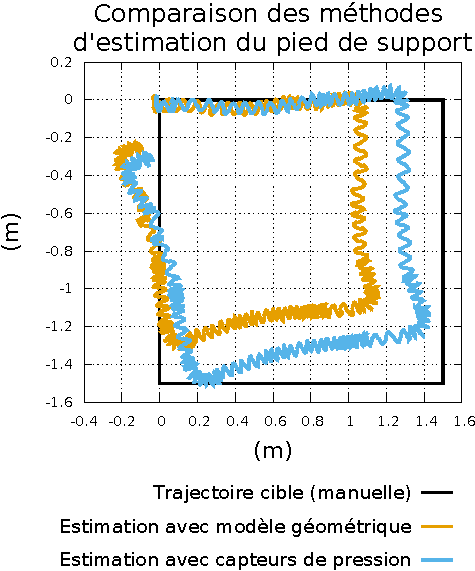
\includegraphics[type=pdf,ext=.pdf,read=.pdf,width=0.75\linewidth]{../plot/odometry_pressure_comparison}
        \end{column}
    \end{columns}
    \begin{block}{}
        \customtextcolor{
            \small
            \textit{Low-cost force sensors for small size humanoid robot}}\\
        \scriptsize
        Grégoire Passault, Quentin Rouxel, Ludovic Hofer, Steve N'Guyen, Olivier Ly\\
        Video contribution, Humanoids, 2015\\
    \end{block}
\end{frame}

\begin{frame}{Imperfections de l'odométrie}
    \begin{columns}
        \begin{column}[T]{0.45\linewidth}
            Erreurs systématiques :
            \begin{itemize}
                \setlength\itemsep{0.5em}
                \item Déformations mécaniques
                \item Latence bas niveau
                \item Filtrage IMU
                \item Erreurs d'asservissement
            \end{itemize}
        \end{column}
        \begin{column}[T]{0.45\linewidth}
            Erreurs non systématiques :
            \begin{itemize}
                \setlength\itemsep{0.5em}
                \item Double support
                \item Glissements (sens de l'herbe)
                \item Collisions entre robots
            \end{itemize}
        \end{column}
    \end{columns}
\end{frame}


\section{Correction de l'odométrie : régression et mesure externe}

\begin{frame}{Correction de l'odométrie}
    \tableofcontents[ 
        sectionstyle=show/shaded, 
        subsectionstyle=show/shaded, 
        currentsubsection, 
        hideothersubsections, 
    ] 
\end{frame}


\begin{frame}{Système de mesure externe}
    \begin{columns}
        \begin{column}{0.5\linewidth}
            \begin{block}{Capture de mouvements (\textit{mocap})}
                Mesure externe de la pose absolue 
            \end{block}
            \begin{itemize}
                \item Haute fréquence ($100$~Hz)
                \item Bonne précision (millimètre)
            \end{itemize}
            Mais :
            \begin{itemize}
                \item Matériel \og encombrant \fg
            \end{itemize}
            \vspace{1em}
            $\Longrightarrow$ Mesure déplacements égocentriques
        \end{column}
        \begin{column}{0.5\linewidth}
            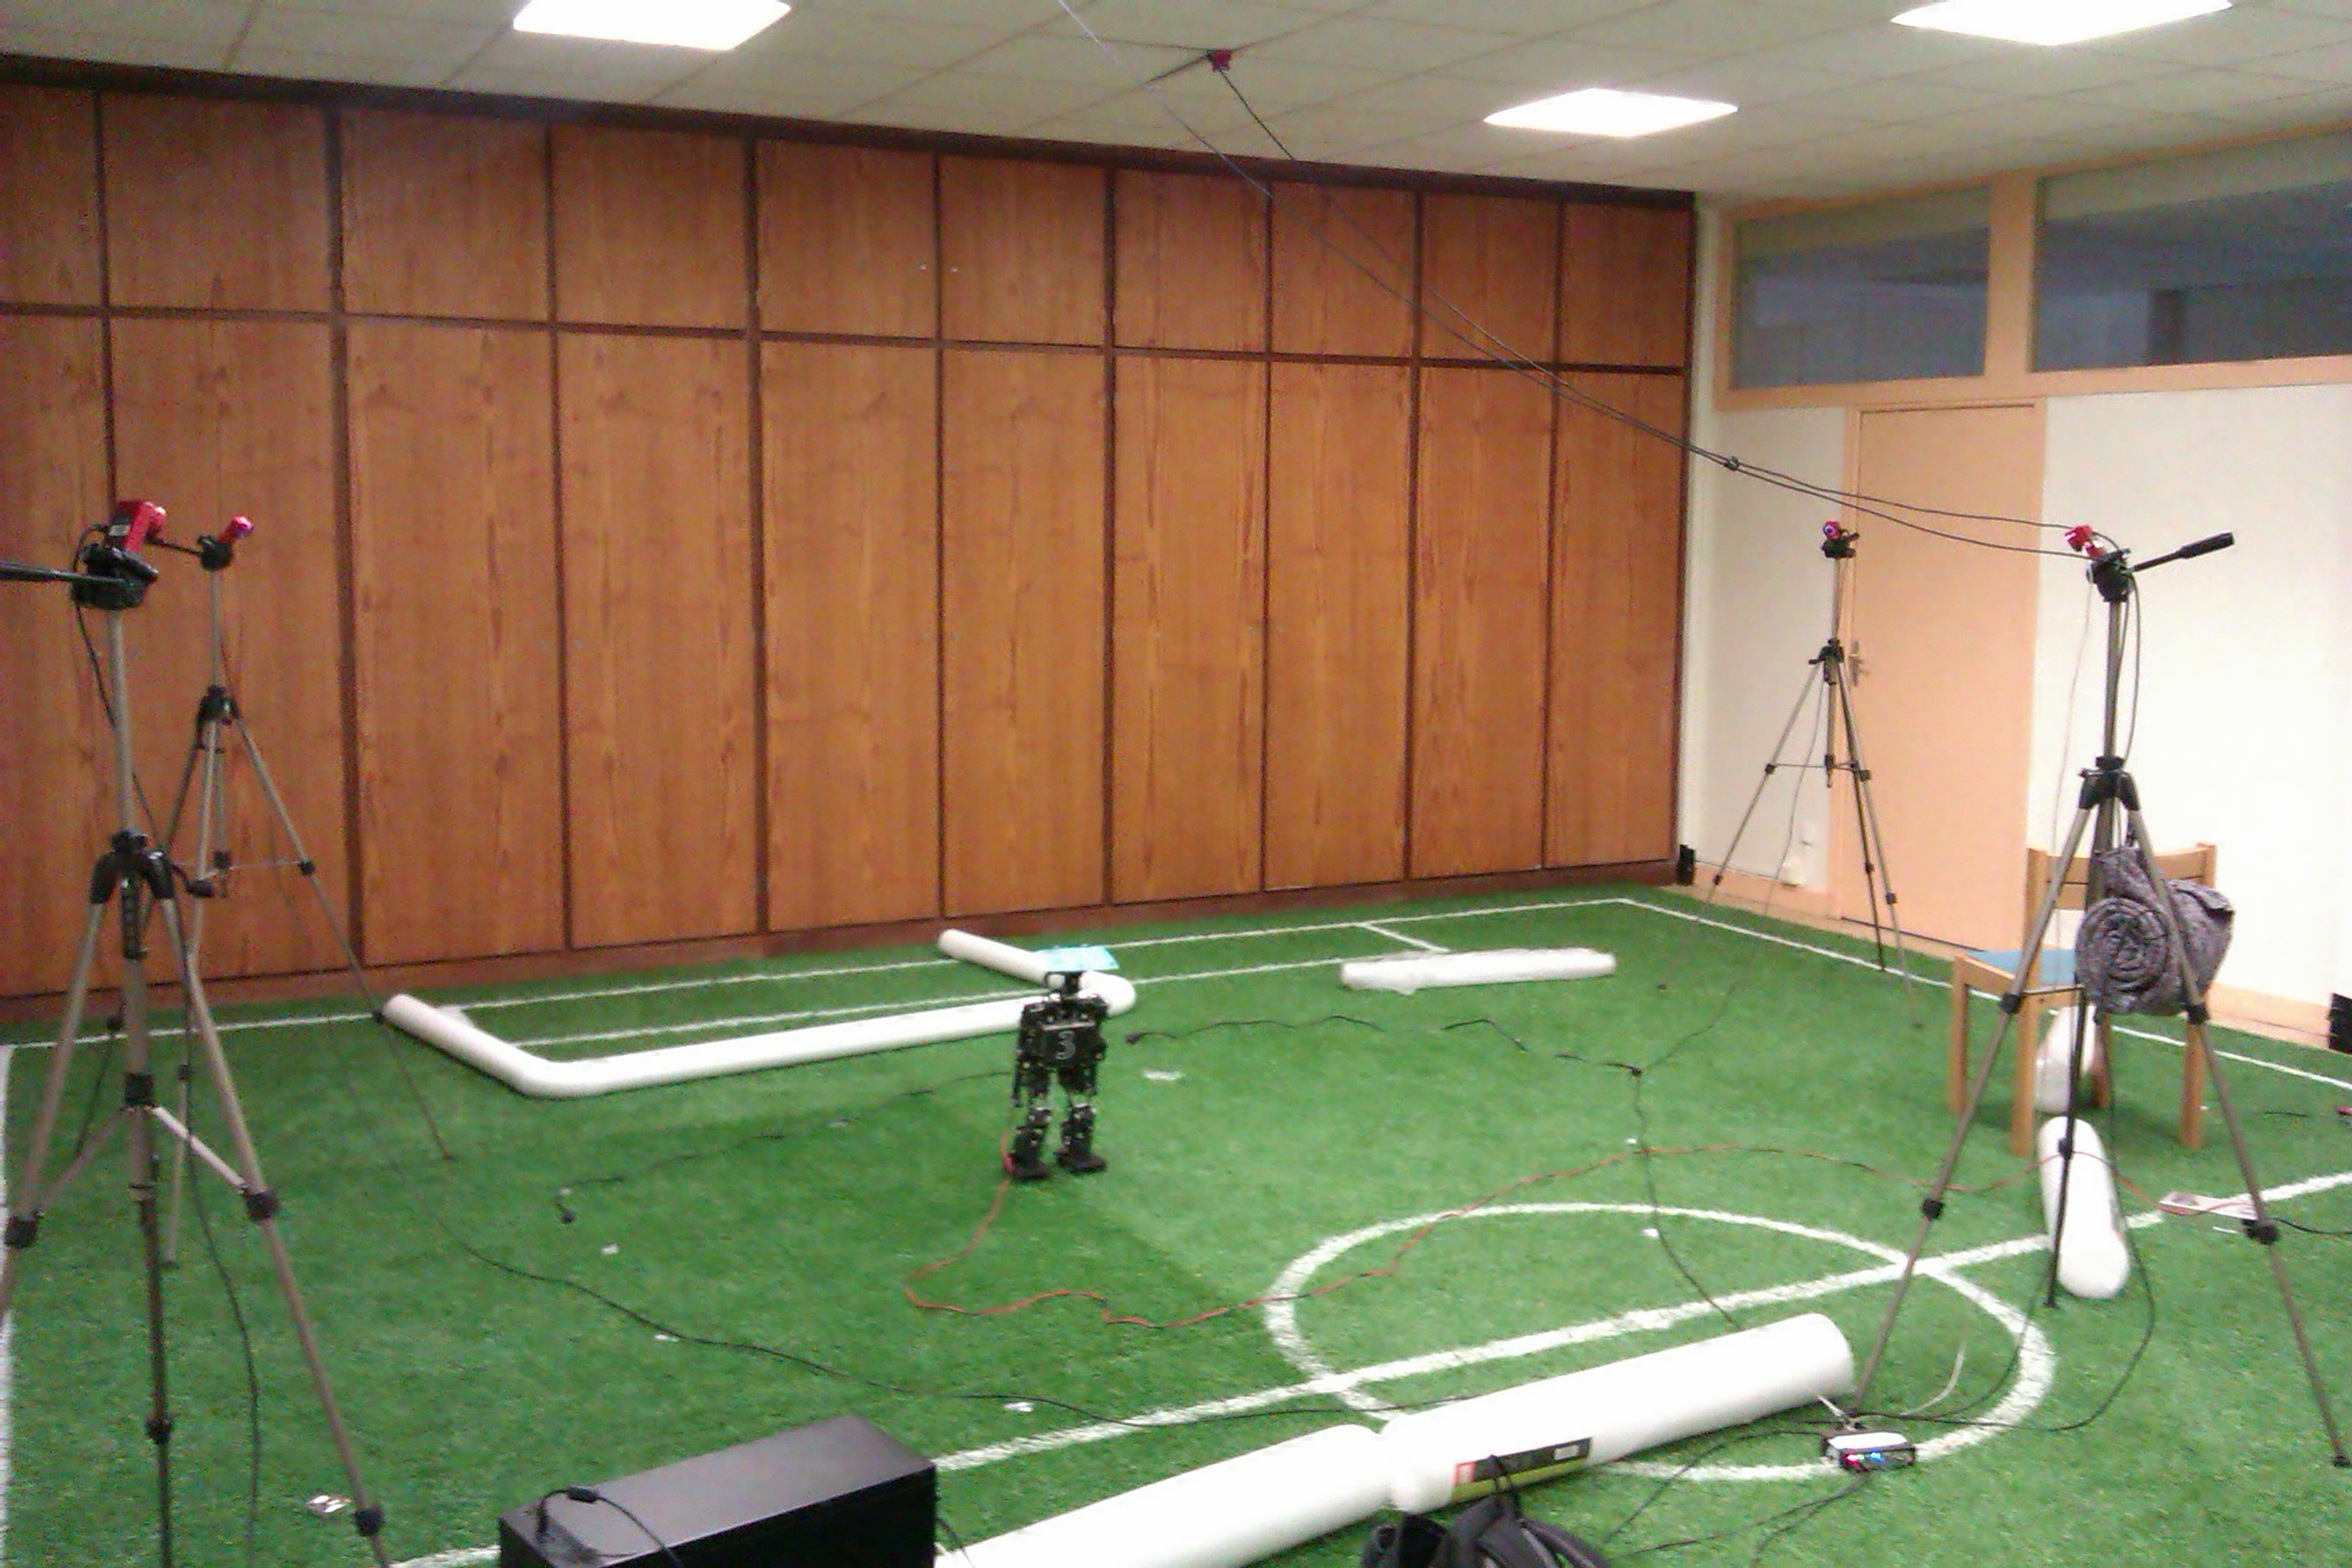
\includegraphics[width=1.0\linewidth]{../media/mocap_setup1.jpg}
        \end{column}
    \end{columns}
\end{frame}

\begin{frame}{Apprentissage des fonctions de correction}
    $\Delta \bm{p}_{t}^{\text{read}} \in \mathbb{R}^3$ : estimation déplacement égocentrique proprioceptive au pas $t$\\
    $\Delta \bm{p}_{t}^{\text{mocap}} \in \mathbb{R}^3$ : mesure déplacement égocentrique au pas $t$\\
    $s_{t}^{\text{read}} \in \{0, 1\}$ : pied de support proprioceptif au pas $t$\\
    $l_{t} \in \mathbb{R}_{+}$ : durée du pas $t$\\
    \vspace{1em}
    Odométrie proprioceptive :
    $$
    \mathbb{R}^9 \longrightarrow \mathbb{R}
    $$
    $$
    \begin{cases}
    \big(\Delta \bm{p}_{t}^{\text{read}}, \Delta \bm{p}_{t-1}^{\text{read}}, s_{t}^{\text{read}}, l_{t}, l_{t-1}\big) 
    \longmapsto \Delta x_{t}^{\text{mocap}} \\
    \big(\Delta \bm{p}_{t}^{\text{read}}, \Delta \bm{p}_{t-1}^{\text{read}}, s_{t}^{\text{read}}, l_{t}, l_{t-1}\big) 
    \longmapsto \Delta y_{t}^{\text{mocap}} \\
    \big(\Delta \bm{p}_{t}^{\text{read}}, \Delta \bm{p}_{t-1}^{\text{read}}, s_{t}^{\text{read}}, l_{t}, l_{t-1}\big) 
    \longmapsto \Delta \theta_{t}^{\text{mocap}} \\
    \end{cases}
    $$
    Odométrie prédictive :
    $$
    \mathbb{R}^7 \longrightarrow \mathbb{R}
    $$
    $$
    \begin{cases}
    \big(\Delta \bm{p}_{t}^{\text{goal}}, \Delta \bm{p}_{t-1}^{\text{goal}}, s_{t}^{\text{goal}}\big) 
    \longmapsto \Delta x_{t}^{\text{mocap}} \\
    \big(\Delta \bm{p}_{t}^{\text{goal}}, \Delta \bm{p}_{t-1}^{\text{goal}}, s_{t}^{\text{goal}}\big) 
    \longmapsto \Delta y_{t}^{\text{mocap}} \\
    \big(\Delta \bm{p}_{t}^{\text{goal}}, \Delta \bm{p}_{t-1}^{\text{goal}}, s_{t}^{\text{goal}}\big) 
    \longmapsto \Delta \theta_{t}^{\text{mocap}} \\
    \end{cases}
    $$
\end{frame}

\begin{frame}{Régression non paramétrique LWPR}
    \begin{columns}
        \begin{column}{0.7\linewidth}
            \begin{block}{Régression non paramétrique}
                \begin{itemize}
                    \item Pas de forme imposée de la solution
                    \item Nécessite plus de données
                \end{itemize}
            \end{block}
            \vspace{1.0em}
            \textit{Locally Weighted Projection Regression} (LWPR) :
            \begin{itemize}
                \item \customtextcolor{(Vijayakumar et al., 2005)}
                \item Très peu calculatoire
                \item Réduction de dimension
            \end{itemize}
        \end{column}
    \end{columns}
\end{frame}

\begin{frame}{Contextes et expérimentations}
    \begin{columns}
        \begin{column}{0.5\linewidth}
            \vspace{1.0em}
            \begin{itemize}
                \item Herbe artificielle
                \item Pilotage manuel du déplacement
                \item Exploration de l'espace de contrôle
            \end{itemize}
            \vspace{2.0em}
            \centering
            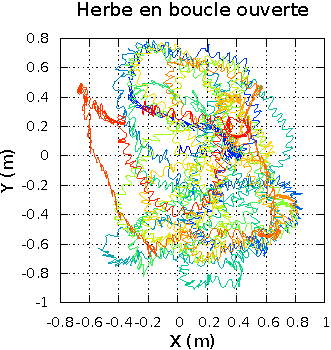
\includegraphics[type=pdf,ext=.pdf,read=.pdf,width=0.8\linewidth]{../plot/OdometryLWPR/grass_open_learn_log_complete_traj}
        \end{column}
        \begin{column}{0.5\linewidth}
            \centering
            \movie[
                autostart,
                width=\linewidth, 
                height=0.56\linewidth,
                poster,
                loop
            ]{}{../video/cutExploreICRA.mp4}
        \end{column}
    \end{columns}
\end{frame}

\begin{frame}{Résultats (1/3) -- Données et corrélations}
    \begin{columns}
        \begin{column}{0.35\linewidth}
            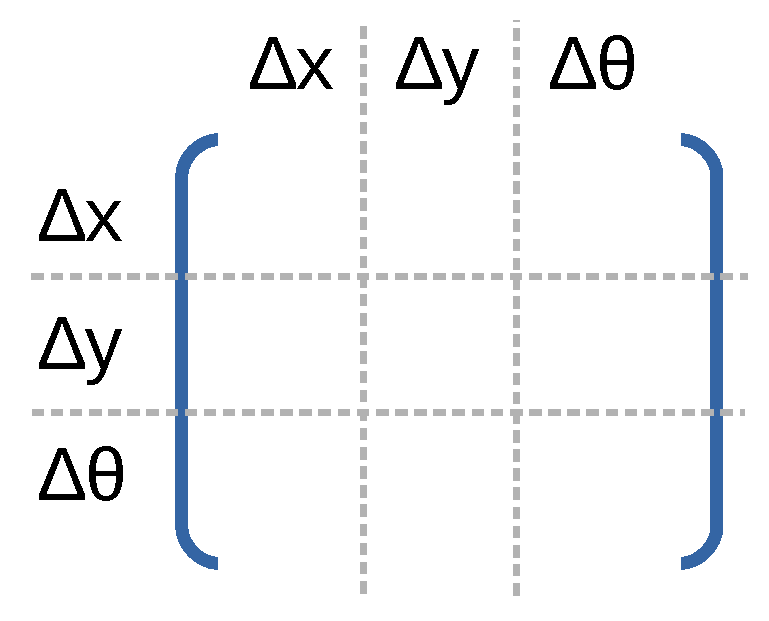
\includegraphics[type=pdf,ext=.pdf,read=.pdf,width=0.8\linewidth]{../schema/correlation_matrix}
        \end{column}
        \begin{column}{0.65\linewidth}
            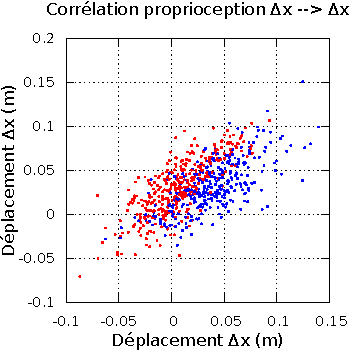
\includegraphics[type=pdf,ext=.pdf,read=.pdf,width=2.5cm]{../plot/OdometryLWPR/grass_close_function_read_x_x}
            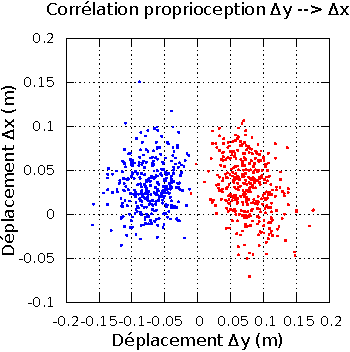
\includegraphics[type=pdf,ext=.pdf,read=.pdf,width=2.5cm]{../plot/OdometryLWPR/grass_close_function_read_y_x}
            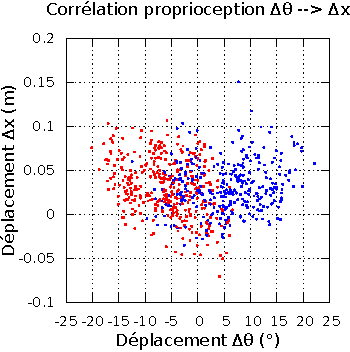
\includegraphics[type=pdf,ext=.pdf,read=.pdf,width=2.5cm]{../plot/OdometryLWPR/grass_close_function_read_yaw_x}
            \vspace{0.2cm}
            \newline
            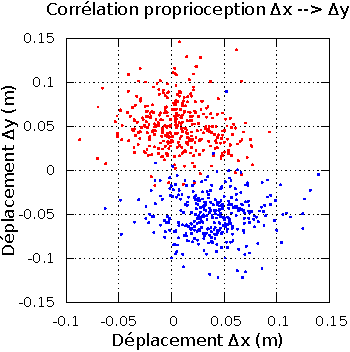
\includegraphics[type=pdf,ext=.pdf,read=.pdf,width=2.5cm]{../plot/OdometryLWPR/grass_close_function_read_x_y}
            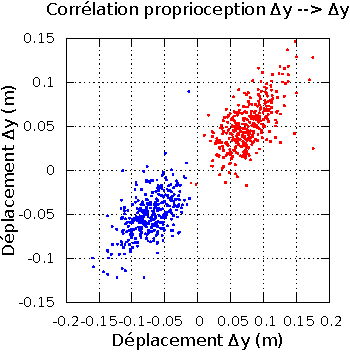
\includegraphics[type=pdf,ext=.pdf,read=.pdf,width=2.5cm]{../plot/OdometryLWPR/grass_close_function_read_y_y}
            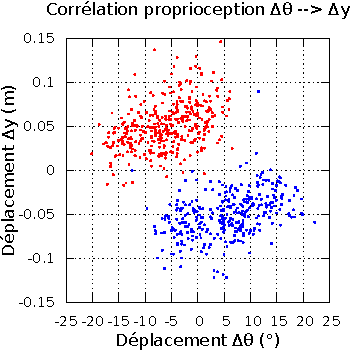
\includegraphics[type=pdf,ext=.pdf,read=.pdf,width=2.5cm]{../plot/OdometryLWPR/grass_close_function_read_yaw_y}
            \vspace{0.2cm}
            \newline
            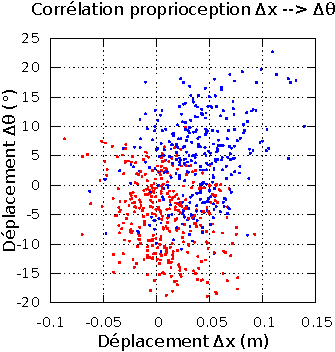
\includegraphics[type=pdf,ext=.pdf,read=.pdf,width=2.5cm]{../plot/OdometryLWPR/grass_close_function_read_x_yaw}
            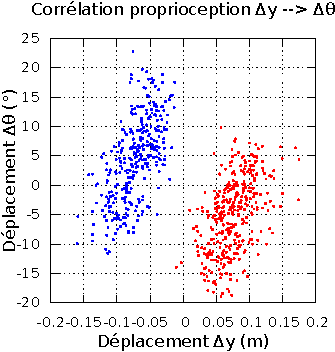
\includegraphics[type=pdf,ext=.pdf,read=.pdf,width=2.5cm]{../plot/OdometryLWPR/grass_close_function_read_y_yaw}
            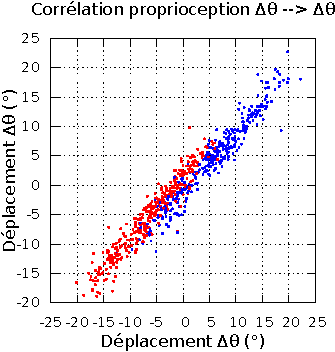
\includegraphics[type=pdf,ext=.pdf,read=.pdf,width=2.5cm]{../plot/OdometryLWPR/grass_close_function_read_yaw_yaw}
        \end{column}
    \end{columns}
\end{frame}

\begin{frame}{Résultats (2/3) -- Trajectoires estimées et statistiques}
    \begin{columns}
        \begin{column}{0.5\linewidth}
            \centering
            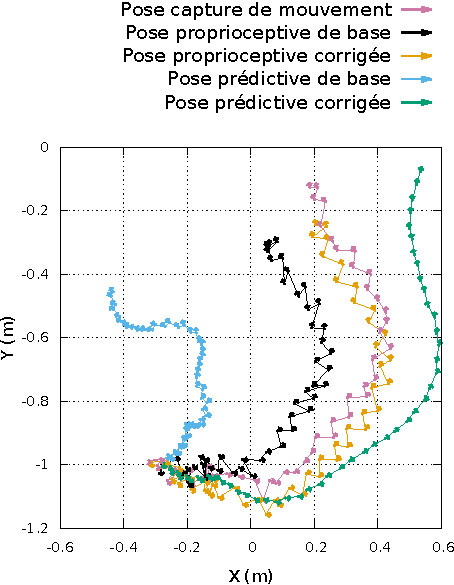
\includegraphics[type=pdf,ext=.pdf,read=.pdf,width=1.0\linewidth]{../plot/OdometryLWPR/grass_open_traj2_pose}
        \end{column}
        \begin{column}{0.5\linewidth}
            \centering
            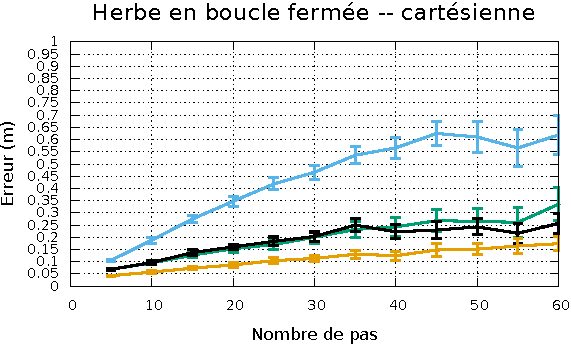
\includegraphics[type=pdf,ext=.pdf,read=.pdf,width=1.0\linewidth]{../plot/OdometryLWPR/grass_close_compare_cart}
            \begin{itemize}
                \item Fonctions de correction $\Rightarrow$ réduction de la dérive
                \item Temps de calcul embarqué (modèle + LWPR) : $8$~ms
            \end{itemize}
        \end{column}
    \end{columns}
\end{frame}

\begin{frame}{Conclusion}
    \begin{columns}
        \begin{column}{0.4\linewidth}
            Comparaison odométrie (40 pas) :
            \begin{itemize}
                \item Proprioceptive corrigée : $0.34$~m $\Rightarrow$ $\bm{0.12}$~m
                \item Visuelle \customtextcolor{(Oriolo at al., 2016)} $\Rightarrow$ $\bm{0.03}$~m
            \end{itemize}
            \vspace{1.0em}
            Cas d'utilisation :
            \begin{itemize}
                \item Temps de calcul
                \item Environnement visuel non adapté
                \item Prédiction (modèle de déplacement) :\\
                    $0.70$~m $\Rightarrow$ $\bm{0.16}$~m
            \end{itemize}
        \end{column}
        \begin{column}{0.6\linewidth}
            \centering
            \movie[
                autostart,
                width=\linewidth, 
                height=0.56\linewidth,
                poster,
                loop
            ]{}{../video/cutICRA_light.mp4}
            \scriptsize
            \definecolor{customCyan}{RGB}{6,206,200}
            \definecolor{customPurple}{RGB}{187,11,231}
            \definecolor{customBlue}{RGB}{9,124,228}
            \definecolor{customGreen}{RGB}{10,188,17}
            \definecolor{customRed}{RGB}{237,12,13}
            \newline
            \vspace{1.0em}
            \begin{tabular}{ll}
                \tikz \fill [customRed]    (0,0) rectangle (0.4,0.2); Mesure & \\
                \tikz \fill [customBlue]   (0,0) rectangle (0.4,0.2); Proprioception base &
                \tikz \fill [customGreen]  (0,0) rectangle (0.4,0.2); Proprioception corrigée\\
                \tikz \fill [customCyan]   (0,0) rectangle (0.4,0.2); Prédiction base &
                \tikz \fill [customPurple] (0,0) rectangle (0.4,0.2); Prédiction corrigée\\
            \end{tabular}
        \end{column}
    \end{columns}
    \begin{block}{}
        \customtextcolor{
            \small
            \textit{Learning the odometry on a small humanoid robot}}\\
        \scriptsize
        Quentin Rouxel, Grégoire Passault, Ludovic Hofer, Steve N'Guyen, Olivier Ly\\
        ICRA, 2016
    \end{block}
\end{frame}



\section{Correction de l'odométrie : modèle linéaire et idendification}

\begin{frame}{Correction de l'odométrie}
    \tableofcontents[ 
        sectionstyle=show/shaded, 
        subsectionstyle=show/shaded, 
        currentsubsection, 
        hideothersubsections, 
    ] 
\end{frame}


\begin{frame}{Modèles linéaires de correction}
    $$
    \mathsf{modeleCorrection} : \Delta \bm{p}_{\text{base}} \in \mathbb{R}^{3} 
    \longmapsto 
    \Delta \bm{p}_{\text{corrigé}} \in \mathbb{R}^{3}
    $$
    \vspace{1em}
    $$
    \only<1>{
        \begin{bmatrix}
            a_{0,0} & a_{0,1} & a_{0,2} & a_{0,3} \\
            a_{1,0} & a_{1,1} & a_{1,2} & a_{1,3} \\
            a_{2,0} & a_{2,1} & a_{2,2} & a_{2,3}
        \end{bmatrix}
    }
    \only<2>{
        \begin{bmatrix}
            0 & \textcolor[rgb]{1,0,0}{a_{0,1}} & 0 & 0 \\
            0 & 0 & \textcolor[rgb]{1,0,0}{a_{1,2}} & 0 \\
            0 & 0 & 0 & \textcolor[rgb]{1,0,0}{a_{2,3}}
        \end{bmatrix}
    }
    \only<3>{
        \begin{bmatrix}
            \textcolor[rgb]{1,0,0}{a_{0,0}} & \textcolor[rgb]{1,0,0}{a_{0,1}} & 0 & 0 \\
            \textcolor[rgb]{1,0,0}{a_{1,0}} & 0 & \textcolor[rgb]{1,0,0}{a_{1,2}} & 0 \\
            \textcolor[rgb]{1,0,0}{a_{2,0}} & 0 & 0 & \textcolor[rgb]{1,0,0}{a_{2,3}}
        \end{bmatrix}
    }
    \only<4>{
        \begin{bmatrix}
            \textcolor[rgb]{1,0,0}{a_{0,0}} & \textcolor[rgb]{1,0,0}{a_{0,1}} & \textcolor[rgb]{1,0,0}{a_{0,2}} & \textcolor[rgb]{1,0,0}{a_{0,3}} \\
            \textcolor[rgb]{1,0,0}{a_{1,0}} & \textcolor[rgb]{1,0,0}{a_{1,1}} & \textcolor[rgb]{1,0,0}{a_{1,2}} & \textcolor[rgb]{1,0,0}{a_{1,3}} \\
            \textcolor[rgb]{1,0,0}{a_{2,0}} & \textcolor[rgb]{1,0,0}{a_{2,1}} & \textcolor[rgb]{1,0,0}{a_{2,2}} & \textcolor[rgb]{1,0,0}{a_{2,3}}
        \end{bmatrix}
    }
    \begin{bmatrix}
        1 \\
        \Delta x_{\text{base}} \\   
        \Delta y_{\text{base}} \\   
        \Delta \theta_{\text{base}}
    \end{bmatrix}
    =
    \begin{bmatrix}
        \Delta x_{\text{corrigé}} \\   
        \Delta y_{\text{corrigé}} \\   
        \Delta \theta_{\text{corrigé}}
    \end{bmatrix}
    =
    \Delta \bm{p}_{\text{corrigé}}
    $$
    \vspace{1em}
    \begin{description}
        \item[Modèle proportionnel] :
            \alt<2>{\textcolor[rgb]{1,0,0}{$3$ paramètres}}{$3$ paramètres}
        \item[Modèle linéaire simple] : 
            \alt<3>{\textcolor[rgb]{1,0,0}{$6$ paramètres}}{$6$ paramètres}
        \item[Modèle linéaire complet] :
            \alt<4>{\textcolor[rgb]{1,0,0}{$12$ paramètres}}{$12$ paramètres}
    \end{description}
    \begin{itemize}
        \item Déplacement sur un cycle de marche (deux pas)
    \end{itemize}
\end{frame}

\begin{frame}{Expérimentation et identification}
    \begin{columns}
        \begin{column}{0.5\linewidth}
            Expérimentations :
            \begin{itemize}
                \item Pas de capteur externe
                \item Mesure manuelle de la pose finale
                \item Peu de séquences (20+5)
            \end{itemize}
            \vspace{1.0em}
            Identification par optimisation\\
            \vspace{1.0em}
            Fonction à minimiser :
            \begin{itemize}
                \item Distance entre poses estimées et observées
            \end{itemize}
        \end{column}
        \begin{column}{0.5\linewidth}
            \centering
            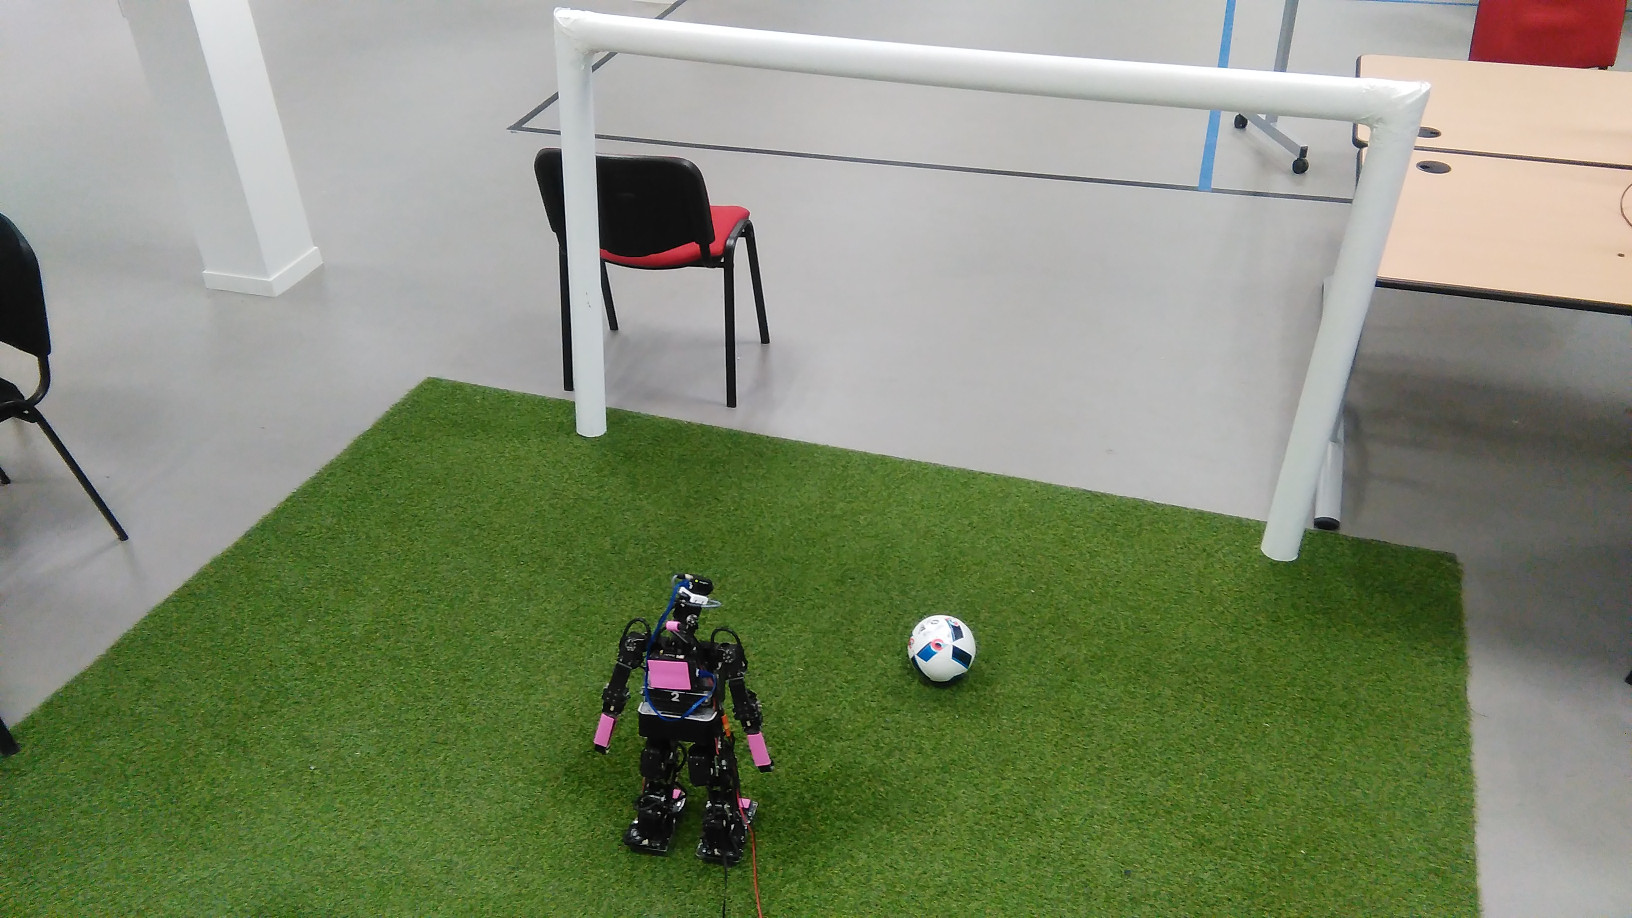
\includegraphics[width=1.0\linewidth]{../media/odometry_cmaes_setup.jpg}
            \vspace{1.0em}
            \small
        \end{column}
    \end{columns}
\end{frame}

\begin{frame}{Optimisation sans gradient}
    \begin{columns}
        \begin{column}{0.5\linewidth}
            \begin{block}{Optimisation sans gradient}
                (boite noire)
                \begin{itemize}
                    \item Fonction non linéaire, non convexe
                    \item Dérivées partielles non connues
                \end{itemize}
            \end{block}
            \vspace{1.0em}
            Covariance Matrix Adaptation Evolution Strategy (CMA-ES) :
            \begin{itemize}
                \item Algorithme génétique
                \item État de l'art \customtextcolor{(Hansen, 2009)}
                \item Implémentation C++ de référence
            \end{itemize}
        \end{column}
        \begin{column}{0.5\linewidth}
            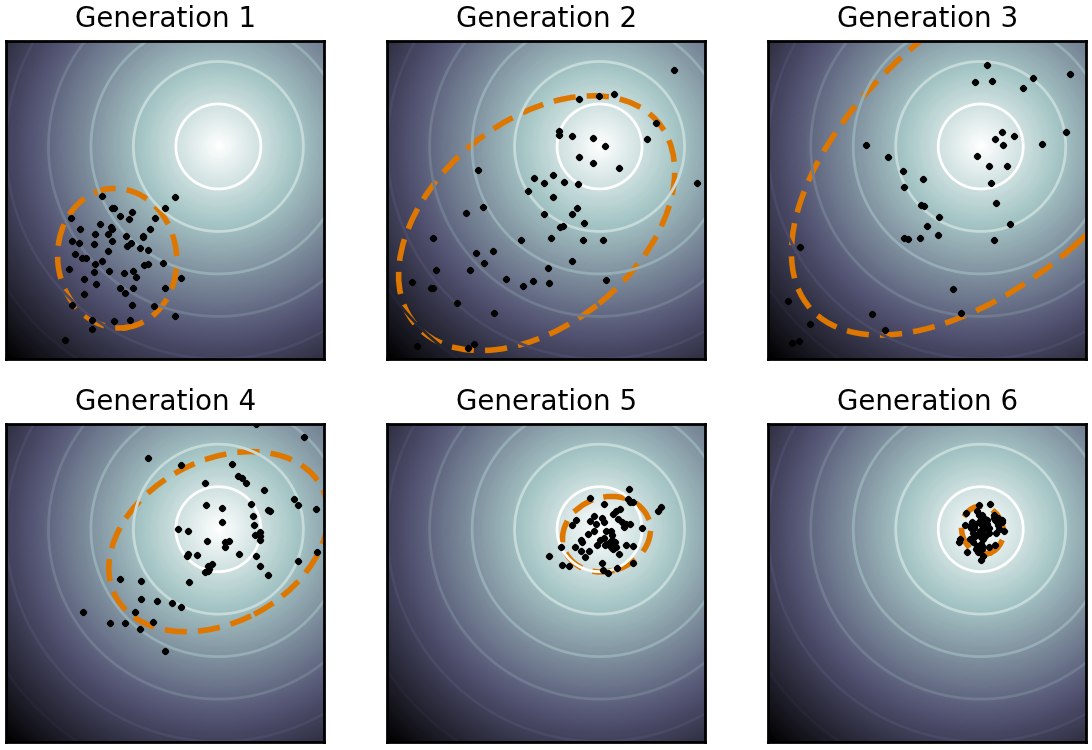
\includegraphics[width=1.0\linewidth]{../media/cmaes.png}\\
            \scriptsize
            (Source : wikipedia)
        \end{column}
    \end{columns}
\end{frame}

\begin{frame}{Résultats -- Comparaison des modèles}
    Après $\approx60$ pas, $20$~s\\
    \vspace{1.0em}
    \begin{columns}
        \begin{column}{0.5\linewidth}
            Odométrie prédictive :\\
            \vspace{1.0em}
            \centering
            \includegraphics[type=pdf,ext=.pdf,read=.pdf,width=1.0\linewidth]{../plot/OdometryCMAES/convergenceOrders}
        \end{column}
        \begin{column}{0.5\linewidth}
            Odométrie proprioceptive :\\
            \vspace{1.0em}
            \centering
            \includegraphics[type=pdf,ext=.pdf,read=.pdf,width=1.0\linewidth]{../plot/OdometryCMAES/convergenceReads}
        \end{column}
    \end{columns}
\end{frame}

\begin{frame}{Conclusion et applications}
    \begin{columns}
        \begin{column}{0.4\linewidth}
            Erreur cartésienne moyenne ($\approx60$ pas) :
            \begin{itemize}
                \item Prédiction :\\
                    $0.39$~m $\Rightarrow$ $\bm{0.27}$~m 
                \item Proprioception :\\
                    $0.21$~m $\Rightarrow$ $\bm{0.11}$~m 
            \end{itemize}
            \vspace{1.0em}
            Odométrie proprioceptive :\\
            $\Longrightarrow$ RoboCup 2016\\
            \vspace{1.0em}
            Odométrie prédictive :\\
            $\Longrightarrow$ Politique de contrôle du déplacement
        \end{column}
        \begin{column}{0.6\linewidth}
            \centering
            \movie[
                autostart,
                width=\linewidth, 
                height=0.56\linewidth,
                poster,
                loop
            ]{}{../video/cutICAPS2017_light.mp4}
        \end{column}
    \end{columns}
    \begin{block}{}
        \customtextcolor{
            \small
            \textit{An operational method toward efficient walk control policies for humanoid robots}}\\
        \scriptsize
        Ludovic Hofer, Quentin Rouxel\\
        ICAPS, 2017
    \end{block}
\end{frame}


\section{Conclusion}

\begin{frame}{Conclusion}
    \tableofcontents[ 
        sectionstyle=show/shaded, 
        subsectionstyle=show/shaded, 
        currentsubsection, 
        hideothersubsections, 
    ] 
\end{frame}


\subsection{Contributions}

\begin{frame}{Résumé des contributions}
    \begin{columns}
        \begin{column}{0.55\linewidth}
            \begin{itemize}
                \item \textbf{Correction de l'odométrie} :
                    \begin{itemize}
                        \item Régression non paramétrique + mesure externe
                        \item Modèle linéaire + optimisation boite noire
                        \item Comparaison proprioception et prédiction
                        \item Comparaison surfaces et stabilisation
                    \end{itemize}
                \item \textbf{Correction du modèle de caméra}
                \item \textbf{Synthèse de mouvements} (en cours) :
                    \begin{itemize}
                        \item Tirs
                        \item Génération par optimisation
                        \item Simulateur physique
                    \end{itemize}
                \item \textbf{Contributions logicielles} :
                    \begin{itemize}
                        \item Ingénierie logicielle ($\approx80000$ lignes)
                        \item Générateurs de marche
                        \item Utilisé par la communauté
                    \end{itemize}
            \end{itemize}
        \end{column}
        \begin{column}{0.45\linewidth}
            \centering
            \movie[
                autostart,
                width=\linewidth, 
                height=0.76\linewidth,
                poster,
                loop
            ]{}{../video/modelKick.ogv}
            \movie[
                autostart,
                width=\linewidth, 
                height=0.56\linewidth,
                poster,
                loop
            ]{}{../video/cutKick_light.mp4}
        \end{column}
    \end{columns}
\end{frame}

\subsection{Perspectives}

\begin{frame}{Perspectives -- Odométrie}
    \begin{itemize}
        \setlength\itemsep{1.0em}
        \item Expérimentation de l'odométrie visuelle
            \begin{itemize}
                \item \customtextcolor{(Oriolo et al., 2016)} mais embarqué
                \item Comparaison sur la même plateforme
                \item Correction proprioception + odométrie visuelle
            \end{itemize}
        \item Modélisation du bruit
            \begin{itemize}
                \item Bruit du déplacement, bruit expérimental
                \item $\Rightarrow$ Maximisation de la vraissamblance
                \item Travaux en cours (\textit{German Open 2017})
            \end{itemize}
        \item Générateur de marche \textit{QuinticWalk}
            \begin{itemize}
                \item Nouvelle marche 2017 plus stable
                \item Moins de bruit
            \end{itemize}
    \end{itemize}
\end{frame}


\subsection{Publications}

\begin{frame}{Publications}
    \begin{itemize}
        \setlength\itemsep{1.0em}
        \item \customtextcolor{
            \small
            \textit{Low-cost force sensors for small size humanoid robot}}\\
            \scriptsize
            Grégoire Passault, Quentin Rouxel, Ludovic Hofer, Steve N'Guyen, Olivier Ly\\
            Video contribution, Humanoids, 2015\\
        \item \customtextcolor{
            \small
            \textit{Rhoban hardware and software open source contributions for robocup humanoids}}\\
            \scriptsize
            Quentin Rouxel, Grégoire Passault, Ludovic Hofer, Steve N'Guyen, Olivier Ly\\
            Workshop on Humanoid Soccer Robots, 2015\\
        \item \customtextcolor{
            \small
            \textit{Learning the odometry on a small humanoid robot}}\\
            \scriptsize
            Quentin Rouxel, Grégoire Passault, Ludovic Hofer, Steve N'Guyen, Olivier Ly\\
            ICRA, 2016\\
        \item \customtextcolor{
            \small
            \textit{Dynaban, an open-source alternative firmware for dynamixel servomotors}}\\
            \scriptsize
            Rémi Fabre, Quentin Rouxel, Grégoire Passault, Steve N'Guyen, Olivier Ly\\
            Symposium RoboCup, 2016\\
        \item \customtextcolor{
            \small
            \textit{Rhoban football club: Robocup humanoid kid-size 2016 champion team paper}}\\
            \scriptsize
            Julien Allali, Louis Deguillaume, Rémi Fabre, Loic Gondry, Ludovic Hofer, Olivier Ly, 
            Steve N'Guyen, Grégoire Passault, Antoine Pirrone, Quentin Rouxel\\
            RoboCup 2016\\
        \item \customtextcolor{
            \small
            \textit{An operational method toward efficient walk control policies for humanoid robots}}\\
            \scriptsize
            Ludovic Hofer, Quentin Rouxel\\
            ICAPS, 2017
    \end{itemize}
\end{frame}



\begin{frame}{}
    \begin{columns}
        \begin{column}{0.7\linewidth}
            \centering
            \movie[
                autostart,
                width=\linewidth, 
                height=0.56\linewidth,
                poster,
                loop
            ]{}{../video/cutRoboCup2017_light.mp4}
        \end{column}
    \end{columns}
    \centering
    \includegraphics[height=3.0cm]{../media/all_robots2.png}
\end{frame}




\begin{frame}[noframenumbering]{}
\end{frame}

\begin{frame}[noframenumbering]{Imperfections -- Chutes de tension ohmiques}
    \begin{columns}
        \begin{column}{0.5\linewidth}
            \centering
            \includegraphics[type=pdf,ext=.pdf,read=.pdf,width=1.0\linewidth]{../schema/electric_bus}
        \end{column}
        \begin{column}{0.5\linewidth}
            \centering
            \includegraphics[type=pdf,ext=.pdf,read=.pdf,width=1.0\linewidth]{../plot/motors_voltage}
        \end{column}
    \end{columns}
    \begin{itemize}
        \item Usure des connecteurs $\Rightarrow$ résistance électrique
        \item Chutes de la tension sur le bus
        \item $\Rightarrow$ Affaiblissement du couple maximum
    \end{itemize}
\end{frame}


\begin{frame}[noframenumbering]{Mouvement de marche}
    \begin{columns}
        \begin{column}{0.4\textwidth}
            \begin{itemize}
                \item Générateur \textit{IKWalk} boucle ouverte + stabilisation
                \item Holonome
                \item Réglage manuel par expérimentation
                \item Mouvement désiré $\neq$ mesuré
                \item Amélioration 2017 : générateur \textit{QuinticWalk}
            \end{itemize}
        \end{column}
        \begin{column}{0.6\textwidth}
            \centering
            \includegraphics[type=pdf,ext=.pdf,read=.pdf,width=1.0\linewidth]{../plot/walk_traj_foot}
        \end{column}
    \end{columns}
    \vspace{0.2cm}
    \begin{block}{}
        \customtextcolor{
            \small
            \textit{Rhoban hardware and software open source contributions for robocup humanoids}}\\
        \scriptsize
        Quentin Rouxel, Grégoire Passault, Ludovic Hofer, Steve N'Guyen, Olivier Ly\\
        Workshop on Humanoid Soccer Robots, 2015\\
    \end{block}
\end{frame}

\begin{frame}[noframenumbering]{Mouvement de marche (2/3) -- Générateur \textit{IKWalk}}
    \centering
    \includegraphics[type=pdf,ext=.pdf,read=.pdf,width=1.0\linewidth]{../schema/ikwalk}
    \begin{block}{}
        \customtextcolor{
            \small
            \textit{Rhoban hardware and software open source contributions for robocup humanoids}}\\
        \scriptsize
        Quentin Rouxel, Grégoire Passault, Ludovic Hofer, Steve N'Guyen, Olivier Ly\\
        Workshop on Humanoid Soccer Robots, 2015\\
    \end{block}
\end{frame}

\begin{frame}[noframenumbering]{Mouvement de marche (3/3) -- Stabilisation}
    \begin{columns}
        \begin{column}{0.5\textwidth}
            \begin{itemize}
                \item Stabilisation latérale
                \item Position du centre de pression
                \item Mise en pause du mouvement
            \end{itemize}
        \end{column}
        \begin{column}{0.5\textwidth}
            \centering
            \movie[
                autostart,
                width=\linewidth, 
                height=0.56\linewidth,
                poster,
                loop
            ]{}{../video/cutStabilization_light.mp4}
            \scriptsize
            (Source : Grégoire Passault)
        \end{column}
    \end{columns}
    \centering
    \includegraphics[type=pdf,ext=.pdf,read=.pdf,width=0.6\linewidth]{../plot/walk_stabilization1}
\end{frame}


\begin{frame}[noframenumbering]{QuinticWalk et ZMP}
    \centering
    \includegraphics[type=pdf,ext=.pdf,read=.pdf,width=1.0\linewidth]{../plot/walk_quintic_zmp}
\end{frame}

\begin{frame}[noframenumbering]{Odométrie et LWPR -- LWPR}
    \centering
    \includegraphics[width=0.6\linewidth]{../media/lwpr.jpg}\\
    \scriptsize
    (Source : Sethu Vijayakumar)
\end{frame}

\begin{frame}[noframenumbering]{Odométrie et LWPR}
    \centering
    \includegraphics[type=pdf,ext=.pdf,read=.pdf,height=8.0cm]{../schema/architecture}
\end{frame}

\begin{frame}[noframenumbering]{Odométrie et LWPR -- Contextes}
    Contextes comparés :
    \begin{itemize}
        \item Surface de marche : 
            \begin{itemize}
                \item moquette
                \item herbe artificielle ($3$~cm)
            \end{itemize}
        \item Processus de stabilisation : 
            \begin{itemize}
                \item désactivé (boucle ouverte)
                \item activé (boucle fermée)
            \end{itemize}
    \end{itemize}
\end{frame}

\begin{frame}[noframenumbering]{Odométrie et LWPR -- Délai de l'IMU}
    \centering
    \includegraphics[type=pdf,ext=.pdf,read=.pdf,width=0.5\linewidth]{../plot/OdometryLWPR/grass_open_delay_imu_uncorrected}
    \includegraphics[type=pdf,ext=.pdf,read=.pdf,width=0.5\linewidth]{../plot/OdometryLWPR/grass_open_delay_imu_corrected}
\end{frame}

\begin{frame}[noframenumbering]{Odométrie et LWPR -- Données}
    \centering
    \includegraphics[type=pdf,ext=.pdf,read=.pdf,width=0.25\linewidth]{../plot/OdometryLWPR/grass_open_learn_log_complete_traj}
    \includegraphics[type=pdf,ext=.pdf,read=.pdf,width=0.25\linewidth]{../plot/OdometryLWPR/grass_close_learn_log_complete_traj}
    \includegraphics[type=pdf,ext=.pdf,read=.pdf,width=0.25\linewidth]{../plot/OdometryLWPR/carpet_open_learn_log_complete_traj}
    \includegraphics[type=pdf,ext=.pdf,read=.pdf,width=0.25\linewidth]{../plot/OdometryLWPR/carpet_close_learn_log_complete_traj}
    \newline
    \includegraphics[type=pdf,ext=.pdf,read=.pdf,width=0.25\linewidth]{../plot/OdometryLWPR/grass_open_learn_log_walk_orders}
    \includegraphics[type=pdf,ext=.pdf,read=.pdf,width=0.25\linewidth]{../plot/OdometryLWPR/grass_close_learn_log_walk_orders}
    \includegraphics[type=pdf,ext=.pdf,read=.pdf,width=0.25\linewidth]{../plot/OdometryLWPR/carpet_open_learn_log_walk_orders}
    \includegraphics[type=pdf,ext=.pdf,read=.pdf,width=0.25\linewidth]{../plot/OdometryLWPR/carpet_close_learn_log_walk_orders}
    \newline
\end{frame}

\begin{frame}[noframenumbering]{Odométrie et LWPR -- Corrélations prédictives}
    \begin{columns}
        \begin{column}{0.35\linewidth}
            \includegraphics[type=pdf,ext=.pdf,read=.pdf,width=0.8\linewidth]{../schema/correlation_matrix}
        \end{column}
        \begin{column}{0.65\linewidth}
            \includegraphics[type=pdf,ext=.pdf,read=.pdf,width=2.5cm]{../plot/OdometryLWPR/grass_close_function_goal_x_x}
            \includegraphics[type=pdf,ext=.pdf,read=.pdf,width=2.5cm]{../plot/OdometryLWPR/grass_close_function_goal_y_x}
            \includegraphics[type=pdf,ext=.pdf,read=.pdf,width=2.5cm]{../plot/OdometryLWPR/grass_close_function_goal_yaw_x}
            \vspace{0.2cm}
            \newline
            \includegraphics[type=pdf,ext=.pdf,read=.pdf,width=2.5cm]{../plot/OdometryLWPR/grass_close_function_goal_x_y}
            \includegraphics[type=pdf,ext=.pdf,read=.pdf,width=2.5cm]{../plot/OdometryLWPR/grass_close_function_goal_y_y}
            \includegraphics[type=pdf,ext=.pdf,read=.pdf,width=2.5cm]{../plot/OdometryLWPR/grass_close_function_goal_yaw_y}
            \vspace{0.2cm}
            \newline
            \includegraphics[type=pdf,ext=.pdf,read=.pdf,width=2.5cm]{../plot/OdometryLWPR/grass_close_function_goal_x_yaw}
            \includegraphics[type=pdf,ext=.pdf,read=.pdf,width=2.5cm]{../plot/OdometryLWPR/grass_close_function_goal_y_yaw}
            \includegraphics[type=pdf,ext=.pdf,read=.pdf,width=2.5cm]{../plot/OdometryLWPR/grass_close_function_goal_yaw_yaw}
        \end{column}
    \end{columns}
\end{frame}

\begin{frame}[noframenumbering]{Odométrie et LWPR -- Convergence}
    \centering
    \includegraphics[type=pdf,ext=.pdf,read=.pdf,width=0.2\linewidth]{../plot/OdometryLWPR/grass_open_convergence_x}
    \includegraphics[type=pdf,ext=.pdf,read=.pdf,width=0.2\linewidth]{../plot/OdometryLWPR/grass_open_convergence_y}
    \includegraphics[type=pdf,ext=.pdf,read=.pdf,width=0.2\linewidth]{../plot/OdometryLWPR/grass_open_convergence_yaw}
    \newline
    \includegraphics[type=pdf,ext=.pdf,read=.pdf,width=0.2\linewidth]{../plot/OdometryLWPR/grass_close_convergence_x}
    \includegraphics[type=pdf,ext=.pdf,read=.pdf,width=0.2\linewidth]{../plot/OdometryLWPR/grass_close_convergence_y}
    \includegraphics[type=pdf,ext=.pdf,read=.pdf,width=0.2\linewidth]{../plot/OdometryLWPR/grass_close_convergence_yaw}
    \newline
    \includegraphics[type=pdf,ext=.pdf,read=.pdf,width=0.2\linewidth]{../plot/OdometryLWPR/carpet_open_convergence_x}
    \includegraphics[type=pdf,ext=.pdf,read=.pdf,width=0.2\linewidth]{../plot/OdometryLWPR/carpet_open_convergence_y}
    \includegraphics[type=pdf,ext=.pdf,read=.pdf,width=0.2\linewidth]{../plot/OdometryLWPR/carpet_open_convergence_yaw}
    \newline
    \includegraphics[type=pdf,ext=.pdf,read=.pdf,width=0.2\linewidth]{../plot/OdometryLWPR/carpet_close_convergence_x}
    \includegraphics[type=pdf,ext=.pdf,read=.pdf,width=0.2\linewidth]{../plot/OdometryLWPR/carpet_close_convergence_y}
    \includegraphics[type=pdf,ext=.pdf,read=.pdf,width=0.2\linewidth]{../plot/OdometryLWPR/carpet_close_convergence_yaw}
    \newline
\end{frame}

\begin{frame}[noframenumbering]{Odométrie et LWPR -- Statistiques}
    \centering
    \includegraphics[type=pdf,ext=.pdf,read=.pdf,width=0.25\linewidth]{../plot/OdometryLWPR/grass_open_compare_cart}
    \includegraphics[type=pdf,ext=.pdf,read=.pdf,width=0.25\linewidth]{../plot/OdometryLWPR/grass_open_compare_angle}
    \newline
    \includegraphics[type=pdf,ext=.pdf,read=.pdf,width=0.25\linewidth]{../plot/OdometryLWPR/grass_close_compare_cart}
    \includegraphics[type=pdf,ext=.pdf,read=.pdf,width=0.25\linewidth]{../plot/OdometryLWPR/grass_close_compare_angle}
    \newline
    \includegraphics[type=pdf,ext=.pdf,read=.pdf,width=0.25\linewidth]{../plot/OdometryLWPR/carpet_open_compare_cart}
    \includegraphics[type=pdf,ext=.pdf,read=.pdf,width=0.25\linewidth]{../plot/OdometryLWPR/carpet_open_compare_angle}
    \newline
    \includegraphics[type=pdf,ext=.pdf,read=.pdf,width=0.25\linewidth]{../plot/OdometryLWPR/carpet_close_compare_cart}
    \includegraphics[type=pdf,ext=.pdf,read=.pdf,width=0.25\linewidth]{../plot/OdometryLWPR/carpet_close_compare_angle}
    \newline
\end{frame}

\begin{frame}[noframenumbering]{Odométrie et LWPR -- Trajectoires}
    \centering
    \includegraphics[type=pdf,ext=.pdf,read=.pdf,width=0.3\linewidth]{../plot/OdometryLWPR/grass_open_traj1_pose}
    \includegraphics[type=pdf,ext=.pdf,read=.pdf,width=0.3\linewidth]{../plot/OdometryLWPR/grass_open_traj2_pose}
    \newline
    \includegraphics[type=pdf,ext=.pdf,read=.pdf,width=0.3\linewidth]{../plot/OdometryLWPR/grass_open_traj3_pose}
    \includegraphics[type=pdf,ext=.pdf,read=.pdf,width=0.3\linewidth]{../plot/OdometryLWPR/grass_open_traj4_pose}
    \newline
    %\includegraphics[type=pdf,ext=.pdf,read=.pdf,width=0.3\linewidth]{../plot/OdometryLWPR/grass_open_traj5_pose}
    %\includegraphics[type=pdf,ext=.pdf,read=.pdf,width=0.3\linewidth]{../plot/OdometryLWPR/grass_open_traj6_pose}
    %\newline
\end{frame}

\begin{frame}[noframenumbering]{Odométrie et LWPR -- Comparaisons}
    \begin{columns}
        \begin{column}{0.4\linewidth}
            \begin{itemize}
                \item Sans correction, proprioception et prédiction : 
                    stabilisation $\Rightarrow$ réduction de la dérive
                \item Sans correction, prédiction : 
                    herbe $\Rightarrow$ augmentation de la dérive
                \item Avec correction, prédiction : 
                    stabilisation $\Rightarrow$ augmentation la dérive
                \item Avec correction, proprioception et prédiction :
                    herbe $\Rightarrow$ réduction (légère) de la dérive
            \end{itemize}
        \end{column}
        \begin{column}{0.6\linewidth}
            \centering
            \includegraphics[type=pdf,ext=.pdf,read=.pdf,width=0.9\linewidth]{../plot/OdometryLWPR/comparison_values}
        \end{column}
    \end{columns}
\end{frame}

\begin{frame}[noframenumbering]{Odométrie et CMA-ES -- Formules}
    $$
    2
    \begin{bmatrix}
        \text{stepGain} \\
        \text{lateralGain} \\
        \text{turnGain} \\
    \end{bmatrix}
    =
    \begin{bmatrix}
        \Delta x_{\text{base}} \\   
        \Delta y_{\text{base}} \\   
        \Delta \theta_{\text{base}}
    \end{bmatrix}
    =
    \Delta \bm{p}_{\text{base}}
    $$
    $$
    \begin{cases}
    \bm{p}_{0} = \begin{bmatrix} 0 & 0 & 0 \end{bmatrix}^{\mathsf{T}} \\
        \bm{p}_{k+1} = \mathsf{displtInt}\big(\bm{p}_{k}, \mathsf{Correction}_{\Theta}(\Delta \bm{p}_{\text{base}, k}) \big) \\
    \end{cases}
    $$
    $$
    \mathsf{erreurAngulaire} : 
    \big( \theta_{\text{final}}, \theta_{\text{mesure}} \big) 
    \longmapsto 
    \begin{cases}
        \mathsf{angleDistance}(\theta_{\text{final}}, \theta_{\text{mesure}})
        \text{ si } \geqslant \frac{2\pi}{12} \\
        0 \text{ sinon} \\
    \end{cases}
    $$
    \begin{gather*}
    \mathsf{fitness} : 
    \big( \bm{p}_{\text{final}}, \bm{p}_{\text{mesure}} \big)
    =
    \big( \begin{bmatrix} x_{\text{final}}\\ y_{\text{final}}\\ \theta_{\text{final}}\\ \end{bmatrix}, 
    \begin{bmatrix} x_{\text{mesure}}\\ y_{\text{mesure}}\\ \theta_{\text{mesure}}\\ \end{bmatrix} \big)
    \longmapsto \\
    (x_{\text{final}} - x_{\text{mesure}})^{2} + (y_{\text{final}} - y_{\text{mesure}})^{2}
    + \big( \alpha.\mathsf{erreurAngulaire}(\theta_{\text{final}}, \theta_{\text{mesure}}) \big)^{2}
    \end{gather*}
    $$
    \underset{\Theta}{\mathrm{arg~min}} 
    \big( \sqrt{\frac{1}{n}\sum_{i} \mathsf{fitness}(\bm{p}_{\text{final}}^{i, \Theta}, \bm{p}_{\text{mesure}}^{i})} \big)
    $$
\end{frame}

\begin{frame}[noframenumbering]{Odométrie et CMA-ES -- Exploration}
    \centering
    \includegraphics[type=pdf,ext=.pdf,read=.pdf,width=0.65\linewidth]{../plot/OdometryCMAES/walk_orders}
\end{frame}

\begin{frame}[noframenumbering]{Odométrie et CMA-ES -- Paramètres 1}
    \begin{columns}
        \begin{column}{0.5\linewidth}
            \centering
            \includegraphics[type=pdf,ext=.pdf,read=.pdf,width=0.6\linewidth]{../plot/OdometryCMAES/parametersPropOrders}
        \end{column}
        \begin{column}{0.5\linewidth}
            \centering
            \includegraphics[type=pdf,ext=.pdf,read=.pdf,width=0.75\linewidth]{../plot/OdometryCMAES/parametersSimpleOrders}
        \end{column}
    \end{columns}
    \centering
\end{frame}

\begin{frame}[noframenumbering]{Odométrie et CMA-ES -- Paramètres 2}
    \centering
    \includegraphics[type=pdf,ext=.pdf,read=.pdf,height=0.85\textheight]{../plot/OdometryCMAES/parametersFullOrders}
\end{frame}

\begin{frame}[noframenumbering]{Odométrie et CMA-ES -- Trajectoires}
    \centering
    \includegraphics[type=pdf,ext=.pdf,read=.pdf,width=0.20\linewidth]{../plot/OdometryCMAES/ordersTraj1}
    \includegraphics[type=pdf,ext=.pdf,read=.pdf,width=0.20\linewidth]{../plot/OdometryCMAES/ordersTraj2}
    \includegraphics[type=pdf,ext=.pdf,read=.pdf,width=0.20\linewidth]{../plot/OdometryCMAES/ordersTraj3}
    \newline
    \includegraphics[type=pdf,ext=.pdf,read=.pdf,width=0.20\linewidth]{../plot/OdometryCMAES/ordersTraj4}
    \includegraphics[type=pdf,ext=.pdf,read=.pdf,width=0.20\linewidth]{../plot/OdometryCMAES/ordersTraj5}
    \includegraphics[type=pdf,ext=.pdf,read=.pdf,width=0.20\linewidth]{../plot/OdometryCMAES/ordersTraj6}
    \newline
    \includegraphics[type=pdf,ext=.pdf,read=.pdf,width=0.20\linewidth]{../plot/OdometryCMAES/ordersTraj7}
    \includegraphics[type=pdf,ext=.pdf,read=.pdf,width=0.20\linewidth]{../plot/OdometryCMAES/ordersTraj8}
    \includegraphics[type=pdf,ext=.pdf,read=.pdf,width=0.20\linewidth]{../plot/OdometryCMAES/ordersTraj9}
    \newline
\end{frame}

\begin{frame}[noframenumbering]{Politique d'approche de la balle}
    \begin{block}{Problème de l'approche}
        \begin{itemize}
            \item Contrôle de la marche 
            \item $\Rightarrow$ position + orientation de tir
            \item Éviter la collision de la balle
        \end{itemize}
    \end{block}
    \begin{itemize}
        \item Optimisation en simulation
        \item Précompensation des défauts
        \item Modèle du bruit de déplacement
    \end{itemize}
    Politiques comparées :
    \begin{itemize}
        \item Approche experte (machine à états)
        \item Approche experte + optimisation CMA-ES
        \item Politique de contrôle MDP continues
    \end{itemize}
\end{frame}

\begin{frame}[noframenumbering]{Odométrie et CMA-ES -- Comparaisons approches}
    Simulation :\\
    \begin{tabular}{|l|c|c|c|}
        \hline
            & \textit{Expert} & \textit{CMA-ES} & \textit{RFPI} \\
        \hline
        Marche holonome     & 31.84      & 14.90  & 11.88      \\
        Marche quasiment non holonome   & 44.12      & 36.18  & 15.97 \\
        \hline
    \end{tabular}
    \vspace{4em}
    \newline
    Réalité :\\
    \begin{tabular}{|l|c|c|c|}
        \hline
            & \textit{Expert} & \textit{CMA-ES} & \textit{RFPI} \\
        \hline
        Marche holonome   & 19.98      & 13.72  & 11.45      \\
        Marche quasiment non holonome & 48.14      & 25.69  & 18.81 \\
        \hline
    \end{tabular}
\end{frame}

\begin{frame}[noframenumbering]{Odométrie et CMA-ES -- Trajectoires approches}
    \centering
    \includegraphics[type=pdf,ext=.pdf,read=.pdf,width=0.65\linewidth]{../plot/OdometryCMAES/robotTrajs}
\end{frame}

\begin{frame}[noframenumbering]{Tir expert 2016}
    \centering
    \includegraphics[type=pdf,ext=.pdf,read=.pdf,width=1.0\linewidth]{../plot/kickgreg_vel}
\end{frame}

\begin{frame}[noframenumbering]{Modélisation dynamique}
    Équation de la dynamique :
    $$
    \begin{cases}
    \bm{H}\bm{\ddot{q}} + \bm{C} - \bm{K}^\T\bm{\lambda} = \bm{\tau} \\
    \bm{K}\bm{\ddot{q}} = \bm{k}
    \end{cases}
    $$
    Contraintes :
    $$
    \bm{K}\bm{\ddot{q}} = \bm{k}
    $$
    Impulsions :
    $$
    \begin{cases}
        \bm{H}(\bm{\dot{q}}_{+}-\bm{\dot{q}}_{-}) - \bm{K}^\T\bm{\Lambda} = \bm{0} \\
    \bm{K}\bm{\dot{q}}_{+} = \bm{0} \\
    \end{cases}
    $$
    Contacts (LCP) :
    $$
    \dot{\bm{\zeta}} = \bm{M}\bm{\lambda} + \bm{d}
    $$
    $$
    \begin{cases}
    \bm{M} = \bm{K}\bm{H}^{-1}\bm{K}^\T & \in \mathbb{R}^{m \times m}\\
    \bm{d} = \bm{K}\bm{H}^{-1}\left(\bm{\tau} - \bm{C}\right) - \bm{k} & \in \mathbb{R}^{m}\\
    \end{cases}
    $$
\end{frame}

\begin{frame}[noframenumbering]{Modélisation des servomoteurs}
    Modèle électrique (linéaire) :
    $$
    U = \tau_{\text{moteur}} \frac{R}{k_{c}} + \omega k_{e}
    $$
    Réduction :
    $$
    r \omega = \dot{q}
    $$
    Couples :
    $$
    \tau_{\text{externe}} = \frac{1}{r} \tau_{\text{moteur}} - \tau_{\text{friction}} - \tau_{\text{inertie}}
    $$
    Inertie :
    $$
    \tau_{\text{inertie}} = J \ddot{q}
    $$
    Frottement :
    $$
    \mathsf{Friction} :~ \dot{q}
    \longmapsto 
    \tau_{\text{friction}}
    =
    \mu_{\text{vis}} \dot{q} 
    + \big( 
    \mu_{\text{break}} \beta 
    + \mu_{\text{coulomb}} (1-\beta) \big) 
    \eta
    $$
    $$
    \beta = e^{-|\frac{\dot{q}}{\mu_{\text{vel}}}|}
    $$
    $$
    \eta = \mathsf{tanh}(\mu_{\text{reg}}\dot{q})
    $$
\end{frame}

\begin{frame}[noframenumbering]{Polynome quintique}
    \centering
    \includegraphics[type=pdf,ext=.pdf,read=.pdf,width=0.6\linewidth]{../plot/quintic_runge}
\end{frame}

\begin{frame}[noframenumbering]{Correction de mouvement}
    \centering
    \begin{tabular}{|l|l|l|}
        \hline
        Mouvement & Erreur moyenne (degrés) & Erreur maximale (degrés) \\
        \hline
        \multicolumn{3}{|c|}{Dans le simulateur (identifié)} \\
        \hline
        Original & 2.56 & 17.9 \\
        Feedforward & 1.20 & 9.61 \\
        Simulateur & 0.45 & 3.21 \\
        \hline
        \multicolumn{3}{|c|}{Sur le robot Sigmaban} \\
        \hline
        Original & 2.46 & 22.1 \\
        Feedforward & 0.88 & 12.0 \\
        Simulateur & 0.71 & 5.94 \\
        \hline
    \end{tabular}
\end{frame}

\begin{frame}[noframenumbering]{Perspectives -- Mouvements}
    \begin{itemize}
        \setlength\itemsep{1.0em}
        \item Amélioration du simulateur
            \begin{itemize}
                \item Glissement
                \item Dynamique impulsive
            \end{itemize}
        \item Étude du tir expert
        \item Transfert vers la réalité
            \begin{itemize}
                \item Identification dynamique
                \item \customtextcolor{(Hanna et Stone, 2017)} $\Rightarrow$ apprentissage
            \end{itemize}
        \item Étude de la modélisation
            \begin{itemize}
                \item Apport de chaque modèle
            \end{itemize}
    \end{itemize}
\end{frame}

\begin{frame}[noframenumbering]{Architecture logicielle}
    \centering
    \includegraphics[width=1.0\linewidth]{../media/code_graph.png}
\end{frame}



\end{document}

